\chapter{Analysis techniques}

\intro{This chapter introduces the necessary toolset to perform the analyses within this thesis. It is organized to follow the common steps of the analyses. First, the generation of simulated events is introduced. Then, details of the top quark reconstruction, the employed multivariate analysis technique, and the template fit is given which are used to estimate the amount of single top quark events within the recorded data. Lastly, the partonic and fiducial objects are defined to which the observed data is unfolded to for comparison with theoretical predictions.}

%##############################################
\section{Event generation}
%##############################################
\label{sec:technique-event-gen}

To compare reconstructed data with theoretical predictions, samples of simulated events are generated from theory and passed through a simulation of the \gls{cms} detector and emulation of its readout. The standard so-called ``FullSimulation'' package~\cite{1742-6596-396-2-022003,1742-6596-664-7-072022} is based on the Geant4 toolkit~\cite{Agostinelli2003250} which provides a detailed simulation of particle trajectories and interactions with the detector material. A fast alternative, the so-called ``FastSimulation'' package, exists within \gls{cms} as well~\cite{fsimRahmat} but has not been used for simulating the detector response in the analyses within this thesis.

The event generation starts with the \glshere{me} of a hard scattering process of interest. \glshere{mc} methods are employed to sample the corresponding cross section integral. The advantage of \gls{mc}-based methods is that the variance of their result decreases as $1/n$ independently of the integral's dimensionality leading to an efficient convergence compared to quadrature-based methods~(e.g. Simpson's rule, Newton-Cotes). A common method to integrate cross sections is given by the \gls{vegas} algorithm~\cite{OHL199913}. It is based on importance sampling where the integral is sampled not uniformly but along an adaptive importance function instead. The resulting sample of events reflects the probability distribution of a process over its phase space. Typically a reweighting is performed in addition such that all events contribute the same probability (e.i. they carry the same absolute weight). 

After obtaining events from the hard interaction, a \glshere{ps} program simulates the hadronization of final state partons. In addition, the radiation of gluons or quarks from initial or final state partons is accounted for as well as contributions from soft secondary interactions, the so-called underlying event, and potential color reconnection effects. A sketch of various parts within an exemplary pp collision event after hadronization is shown in Fig.~\ref{fig:technique-mcevent}. The \gls{ps} simulation is based on Altarelli-Parisi splitting functions~\cite{Altarelli:1977zs} which allow to calculate the probability of soft parton emissions, e.g. $\mathrm{q}\to \mathrm{gq}$. It is convenient to calculate the ``surviving'' probability, the so-called Sudakov factor, that a parton does not branch further below a certain energy scale. During the \gls{ps} simulation a complication arises from potential double counting of soft parton emissions since the simulation of the hard interaction may lead to a soft emission as well which is however already accounted for by the \gls{ps}. These are avoided by applying a \gls{me}-to-\gls{ps} matching scheme which yields a criterion to assign additional emissions to either the simulation of the hard interaction or the \gls{ps} exclusively depending on the event kinematics. A general introduction to parton shower simulation and matching algorithms can be found in Refs.~\cite{Hoche:2014rga,Alwall:2007fs}.

\todo{explain and ref ISR/FSR}


\myfigure{\label{fig:technique-mcevent} A sketch of a generated event from the simulation of the hard interaction and subsequent hadronization through a parton shower. The figure is taken in parts from Ref.~\cite{Hoche:2014rga}.}{
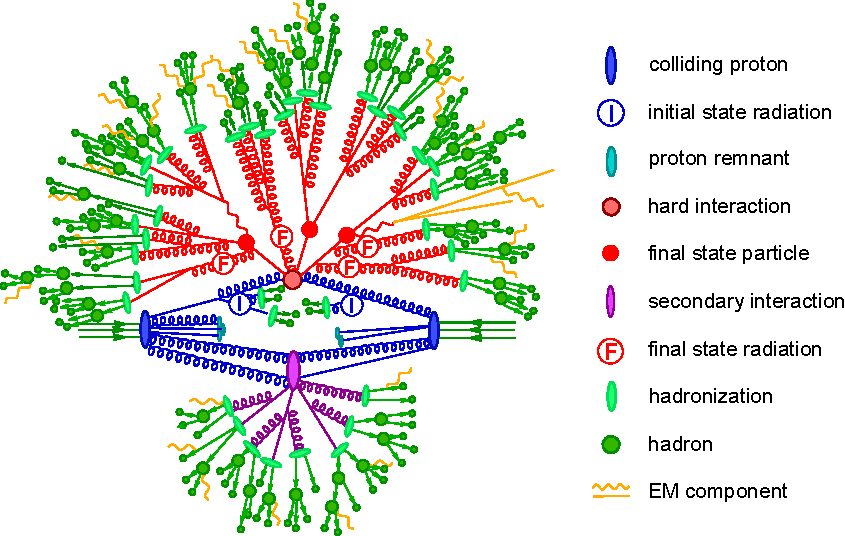
\includegraphics[scale=0.75]{figures/technique/shower.pdf}
}

A brief overview of the programs used for generation and subsequent hadronization of $t$-channel single top quark production is given in the following.

\begin{description}
\item[MadGraph5\_aMC{@}NLO] The \MGAMC[] program~\cite{Alwall:2014hca} is a merge of the \gls{lo} \MG[] generator~\cite{Alwall:2011uj} and \AMC[] into a common framework. It supports the generation of \gls{lo} or \gls{nlo} samples which can be matched to parton showers using the \gls[]{mlm}~\cite{Mangano:2006rw} or MC{@}NLO~\cite{Frixione:2002ik} schemes respectively. The latter method produces a certain fraction of events with negative weights (depending on the process) which stem from a subtraction of additional emissions from the \gls{nlo} matrix element to prevent double-counting. 
Multiple samples of events with additional final state partons at matrix element level can also be merged into a combined sample. Here, the overlap with the \gls{ps} is removed through the \gls[]{fxfx} merging scheme~\cite{Frederix:2012ps}.

\item[Powheg] The \POWHEG[] box (versions~1,2)~\cite{Alioli:2010xd} is a program that contains predefined implementations of various processes such as $t$-channel single top quark production~\cite{Alioli:2009je} at \gls{nlo}. It utilizes the so-called \POWHEG method~\cite{Frixione:2007vw} for matching in which the hardest radiation generated from the \gls{me} has priority over subsequent \gls{ps} emissions. This removes the overlap with the \gls{ps} without the generation of negatively weighted events.

\item[CompHEP] The \COMPHEP[] program (version~4.5)~\cite{Boos:2004kh} can perform calculations of cross sections from Lagrangian densities at \gls{lo}. In addition, generation of events is also possible such as single top quark production~\cite{Boos:2006af}. Here, an approximation is used by combining events from the $2\to2$ and $2\to3$ processes which reproduces effectively \gls{nlo} corrections.

\item[Tauola] Event generators can be interfaced with the \TAUOLA[] library~\cite{Jadach:1993hs,Davidson:2010rw} to simulate leptonic and hadronic decays of tau leptons. It accounts for spin polarization effects while also including the radiation of photons from \gls{qed} corrections by incorporating the \PHOTOS[] library~\cite{Golonka:2005pn}.

\item[MadSpin] The generation of processes involving resonances and their decay products is a computational-intensive task especially at \gls{nlo}. The complexity can be reduced by only simulating an event up to narrow resonance like the top quark or Higgs boson. In the narrow width approximation where a resonant particle is taken to be on-shell, the production and decay factorizes which allows to split the simulation in a production and decay step. The \MADSPIN[] program~\cite{Artoisenet:2012st} extends this approach by also accounting for off-shell effects through a partial reweighting of events. In addition, spin correlations effects are emulated as well.

\item[Pythia] The \PYTHIA[] program (versions~6,8)~\cite{Sjostrand:2006za,Sjostrand:2014zea} can generate events of various processes at \gls{lo}. It is however famous for its \gls{ps} simulation which can be interfaced with other \gls{lo} and \gls{nlo} event generators to perform subsequent parton showering, hadronization, and the simulation of the underlying event. For hadronization, a phenomenological model is utilized in which one-dimensional strings\footnote{The string model is motivated by the fact that the spatial form of a dipole color field does not extend radially like an \gls{em} field but is instead squeezed to a tube-like form.} connected to partons reflect the color field leading to the creation of additional partons through string branching and finally to the formation of color-neutral singlets.

\item[Herwig++] The \HERWIG[] program (version~7)~\cite{Bellm:2015jjp} is an \gls{nlo} event generator which is also capable of simulating the showering of partons similar to \PYTHIA. Its hadronization algorithm utilizes a model in which color-connected quarks are spatially kept together in clusters~\cite{Webber:1983if} which is motivated by the ``preconfinement'' of color~\cite{Amati:1979fg}. If the mass of a cluster is sufficiently high it can decay into lighter clusters with a certain probability. In its final step, a cluster decays then into a pair of hadrons.
\end{description}




%##############################################
\section{Top quark reconstruction}
%##############################################
\label{sec:technique-topreco}

After the reconstruction and selection of analysis objects, a top quark candidate is reconstructed in the presented analyses. Assuming that the top quark decayed leptonically as $\mathrm{t}\to\mathrm{b}\mathrm{W}\to\mathrm{b}\ell\nu$, its energy and momentum is reconstructed by summing the measured 4-momenta of a selected lepton (muon or electron), b-tagged jet, and neutrino candidate. The neutrino candidate itself is reconstructed from the missing transverse energy and the lepton momentum. This is performed by requiring a W~boson mass constraint of $m_\mathrm{W}=80.4~\GeV$~\cite{Olive:2016xmw} on their invariant mass as

\begin{align}
m_\mathrm{W}^2=\colvec{2}{E_\mathrm{W}}{\vec{p}_\mathrm{W}}^{2}&\overset{!}{=}\left[\colvec{2}{E_{\ell}}{\vec{p}_{\ell}}+\colvec{2}{E_{\nu}}{\vec{p}_{\nu}}\right]^{2}\nonumber\\
&=\underbrace{m_{\ell}^2+m_{\nu}^2}_{\approx 0}+\,2\cdot E_{\ell}\,E_{\nu}-\,2\cdot\colvec{3}{p_{\ell,x}}{p_{\ell,y}}{p_{\ell,z}}\cdot\colvec{3}{p_{\nu,\mathrm{T}}\cdot\cos\phi_{\nu}}{p_{\nu,\mathrm{T}}\cdot\sin\phi_{\nu}}{p_{\nu,z}}\,, \label{eq:technique-neutrino-pz-eq}
\end{align}

where the lepton and neutrino are approximated to be massless. Then, one can solve for the unknown $p_{\nu,z}$-component of the neutrino candidate momentum by taking $p_{\nu,\mathrm{T}}$ and $\phi_{\nu}$ from the missing transverse momentum vector $\pvmiss$. After rearranging, the quadratic equation 

\begin{subequations}
\begin{align}
0&=p_{\nu,z}^2-\frac{2\,\xi\,p_{\ell,z}}{E_{\ell}^{2}-p_{\ell,z}^2}\cdot p_{\nu,z}-\frac{\xi^{2}-E_{\ell}^{2}\,p_{\nu,\mathrm{T}}^2}{E_{\ell}^{2}-p_{\ell,z}^2}\\
\xi&=\frac{m_\mathrm{W}^2}{2}+p_{\nu,\mathrm{T}}\,p_{\ell,\mathrm{T}}\cdot\cos\big(\phi_\ell-\phi_\nu\big)
\end{align}
\end{subequations}

is obtained from Eq.~\ref{eq:technique-neutrino-pz-eq} which possesses the solutions

\begin{align}
p_{\nu,z}^{1,2}=\frac{1}{E_{\ell}^{2}-p_{\ell,z}^{2}}\left[\xi\cdot p_{\ell,z}\pm E_{\ell} \sqrt{\xi^2-p_{\nu,\mathrm{T}}^2\big(E_{\ell}^2-p_{\ell,z}^2\big)}~\right]. \label{eq:technique-neutrino-pz}
\end{align}

A detailed derivation and discussion of this result can be found in Ref.~\cite{Chwalek:1416031}. In simulated $t$-channel single-top-quark events this procedure leads to two real solutions in about 65\% of all events that passed the selection. The difference of the two real solutions with respect to the true neutrino $p_{z}$ at parton level is displayed in Fig.~\ref{fig:technique-neutrino-reco}. The plot demonstrates that choosing the solution which has the smallest absolute $|p_{\nu,z}|$ yields on average a neutrino $p_{z}$ which is closest to the true neutrino $p_{z}$ amongst the two real solutions.

\myfigure{\label{fig:technique-neutrino-reco}Differences of the reconstructed neutrino $p_{z}$ with respect to the neutrino $p_{z}$ at parton level in cases of real and complex solutions for simulated events of $t$-channel single-top-quark production.}{
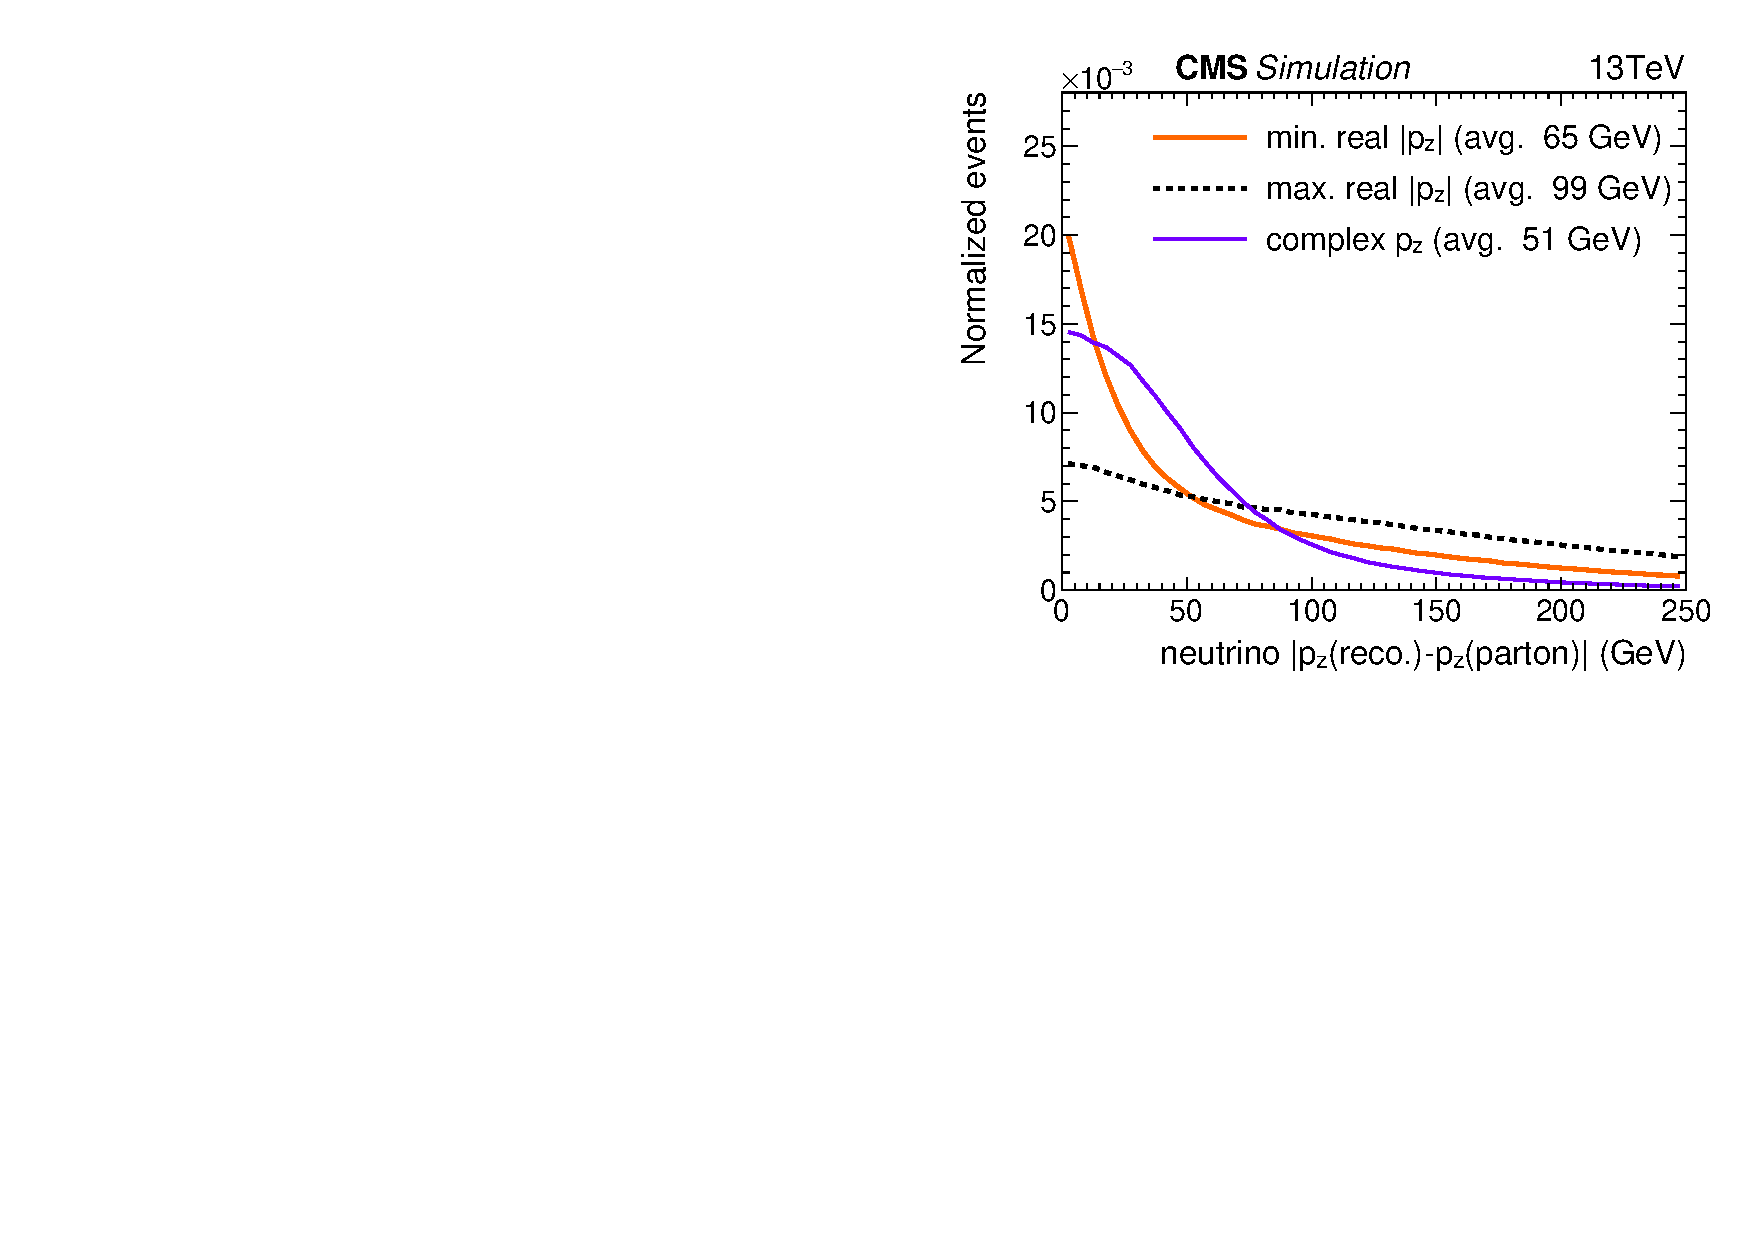
\includegraphics[width=0.52\textwidth]{figures/technique/neutrino_match_dpz.pdf}
}

Complex solutions are obtained if the discriminant in Eq.~\ref{eq:technique-neutrino-pz} becomes negative. This happens for about 35\% of selected signal events. Such solutions occur mostly due to the finite \met resolution whereas the negligence of the W~boson mass width and resolution of the lepton momentum are minor effects. The imaginary part of the solutions is removed by requiring that the discriminant vanishes

\begin{equation}
0\overset{!}{=}\xi^2-p_{\nu,\mathrm{T}}^2\big(E_{\ell}^2-p_{\ell,z}^2\big)\quad
\Rightarrow~ p_{\nu,z}=\frac{\xi\cdot p_{\ell,z}}{E_{\ell}^{2}-p_{\ell,z}^{2}}\,,\label{eq:technique-pz-complex}
\end{equation}

which is equivalent to setting the transverse mass $m_\mathrm{T}$ to the W~boson mass as

\begin{align}
m_\mathrm{W}^2\overset{!}{=}m_\mathrm{T}^2&=(p_{\ell,\mathrm{T}}+p_{\nu,\mathrm{T}})^2-(p_{\ell,x}+p_{\nu,x})^{2}-(p_{\ell,y}+p_{\nu,y})^{2}\nonumber\\
&\approx2\,p_{\ell,\mathrm{T}}^2\,p_{\nu,\mathrm{T}}^2\cdot\Big(1-\cos\big(\phi_\ell-\phi_\nu\big)\Big)\,.
\end{align}

Then, the $p_{\nu,x}$ and $p_{\nu,x}$ components are varied and the pair which minimizes the distance $|\vec{p}_{\nu,\mathrm{T}}-\pvmiss|$ with respect to the measured missing transverse momentum vector is taken as the result. Figure~\ref{fig:technique-neutrino-reco} shows that after removing the imaginary part~(Eq.~\ref{eq:technique-pz-complex}) the $p_{\nu,z}$ solution is on average closer to the true neutrino $p_{\nu,z}$ momentum compared to cases with real solutions. This can be explained as follows. Initially $m_\mathrm{T}>m_\mathrm{W}$ is found in cases of complex solutions which is then modified to $m_\mathrm{T}=m_\mathrm{W}$ by ignoring the imaginary part and applying the minimization procedure as described above. One can therefore argue that this represents a correction of the finite \met resolution which resulted into the complex solutions in the first place.

Finally, after finding a solution for the unknown neutrino $p_{z}$ component, a top quark candidate can be constructed by summing the 4-momenta of the lepton, b-tagged jet, and neutrino candidate. Shape comparisons of the reconstructed top quark mass and pseudorapidity for the two neutrino solution cases are presented in Fig~\ref{fig:technique-top-reco} for simulated signal events. In the case that the initial solution is complex, the reconstruction yields a top quark candidate with an enhanced mass resolution. Similarly, the pseudorapidity of the top quark candidate demonstrates an improved reproduction of the corresponding observable at parton level as well.

\myfigure{\label{fig:technique-top-reco} Shape differences in the reconstructed top quark (a)~mass and (b)~pseudorapidity for cases with real neutrino $p_{z}$ solutions  (where the one with the smallest $|p_{z}|$ is picked) or with initially complex solutions for simulated events of $t$-channel single-top-quark production.}{
\subfloat[]{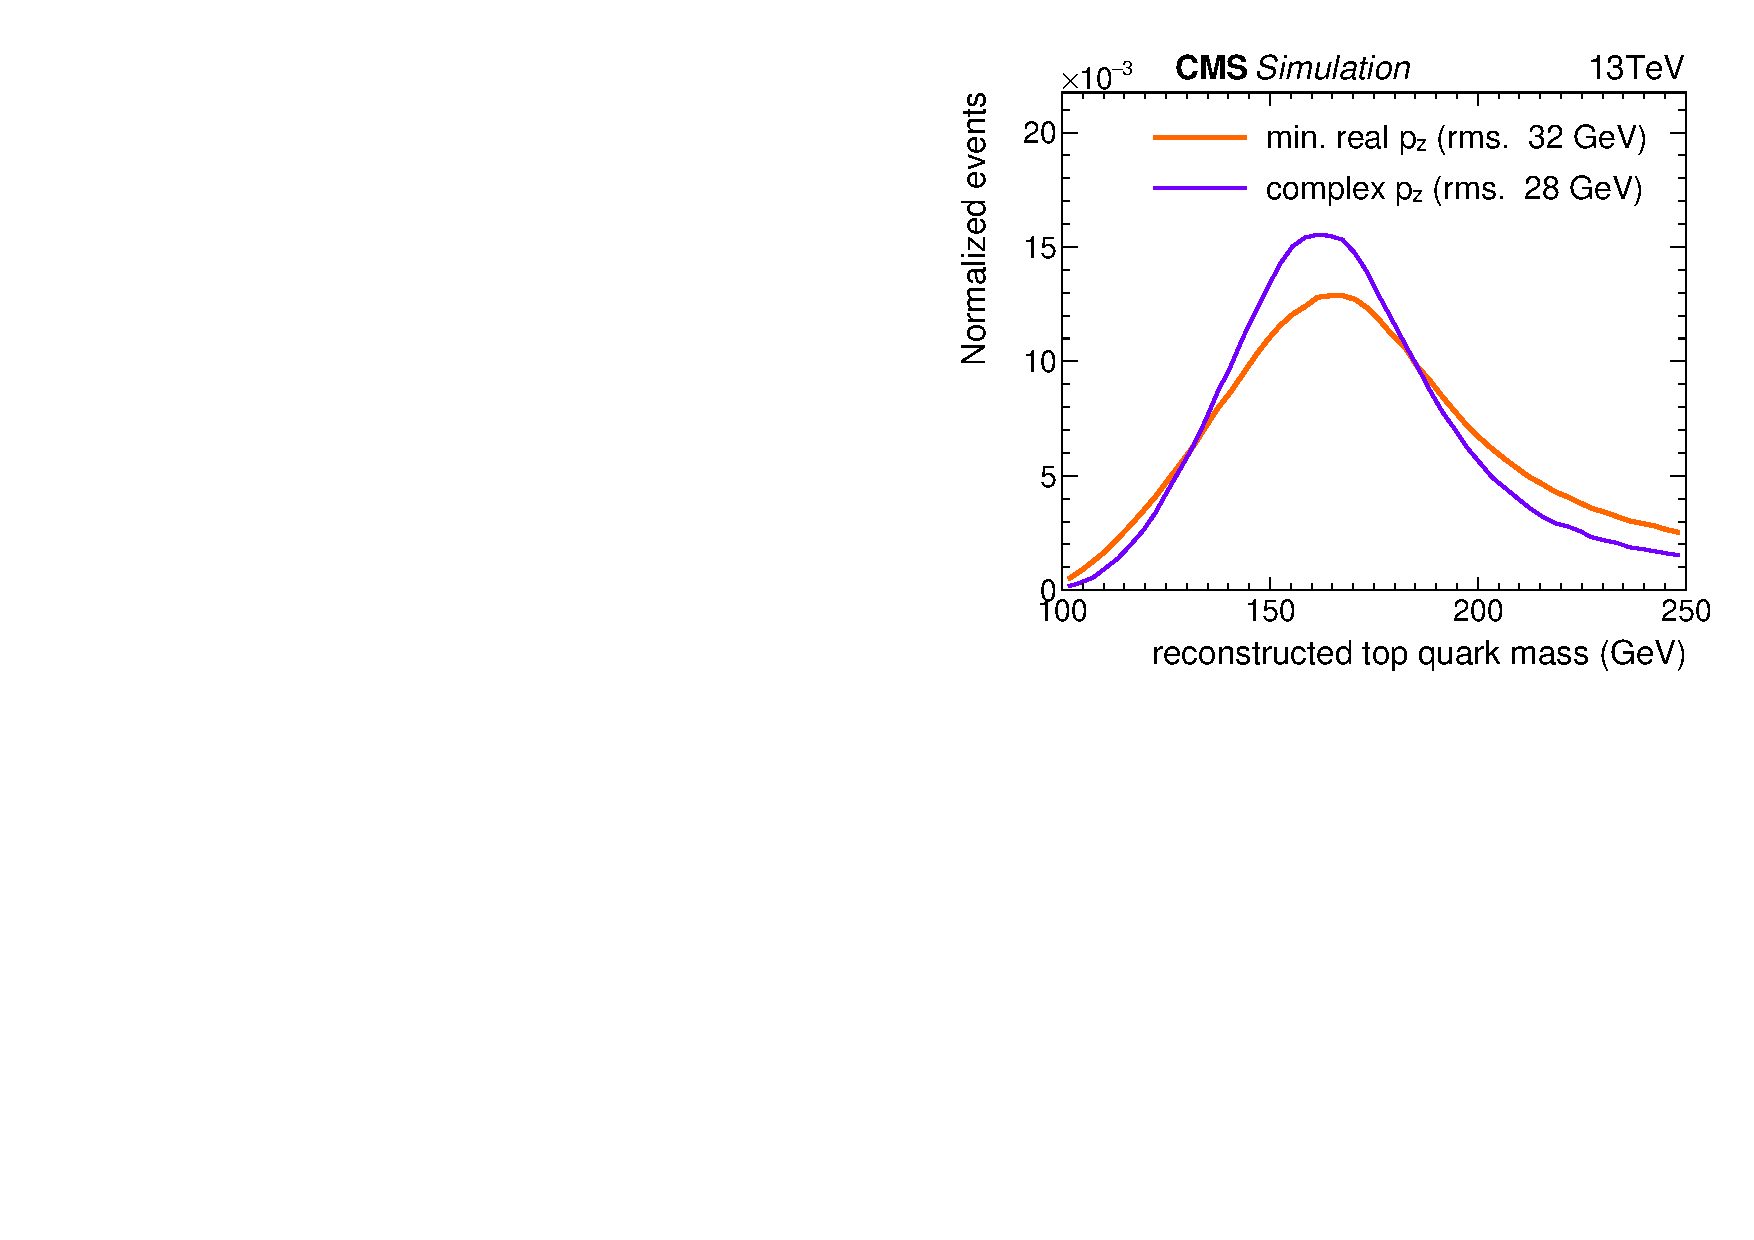
\includegraphics[width=0.48\textwidth]{figures/technique/top_match_mass.pdf}}\hspace{0.03\textwidth}
\subfloat[]{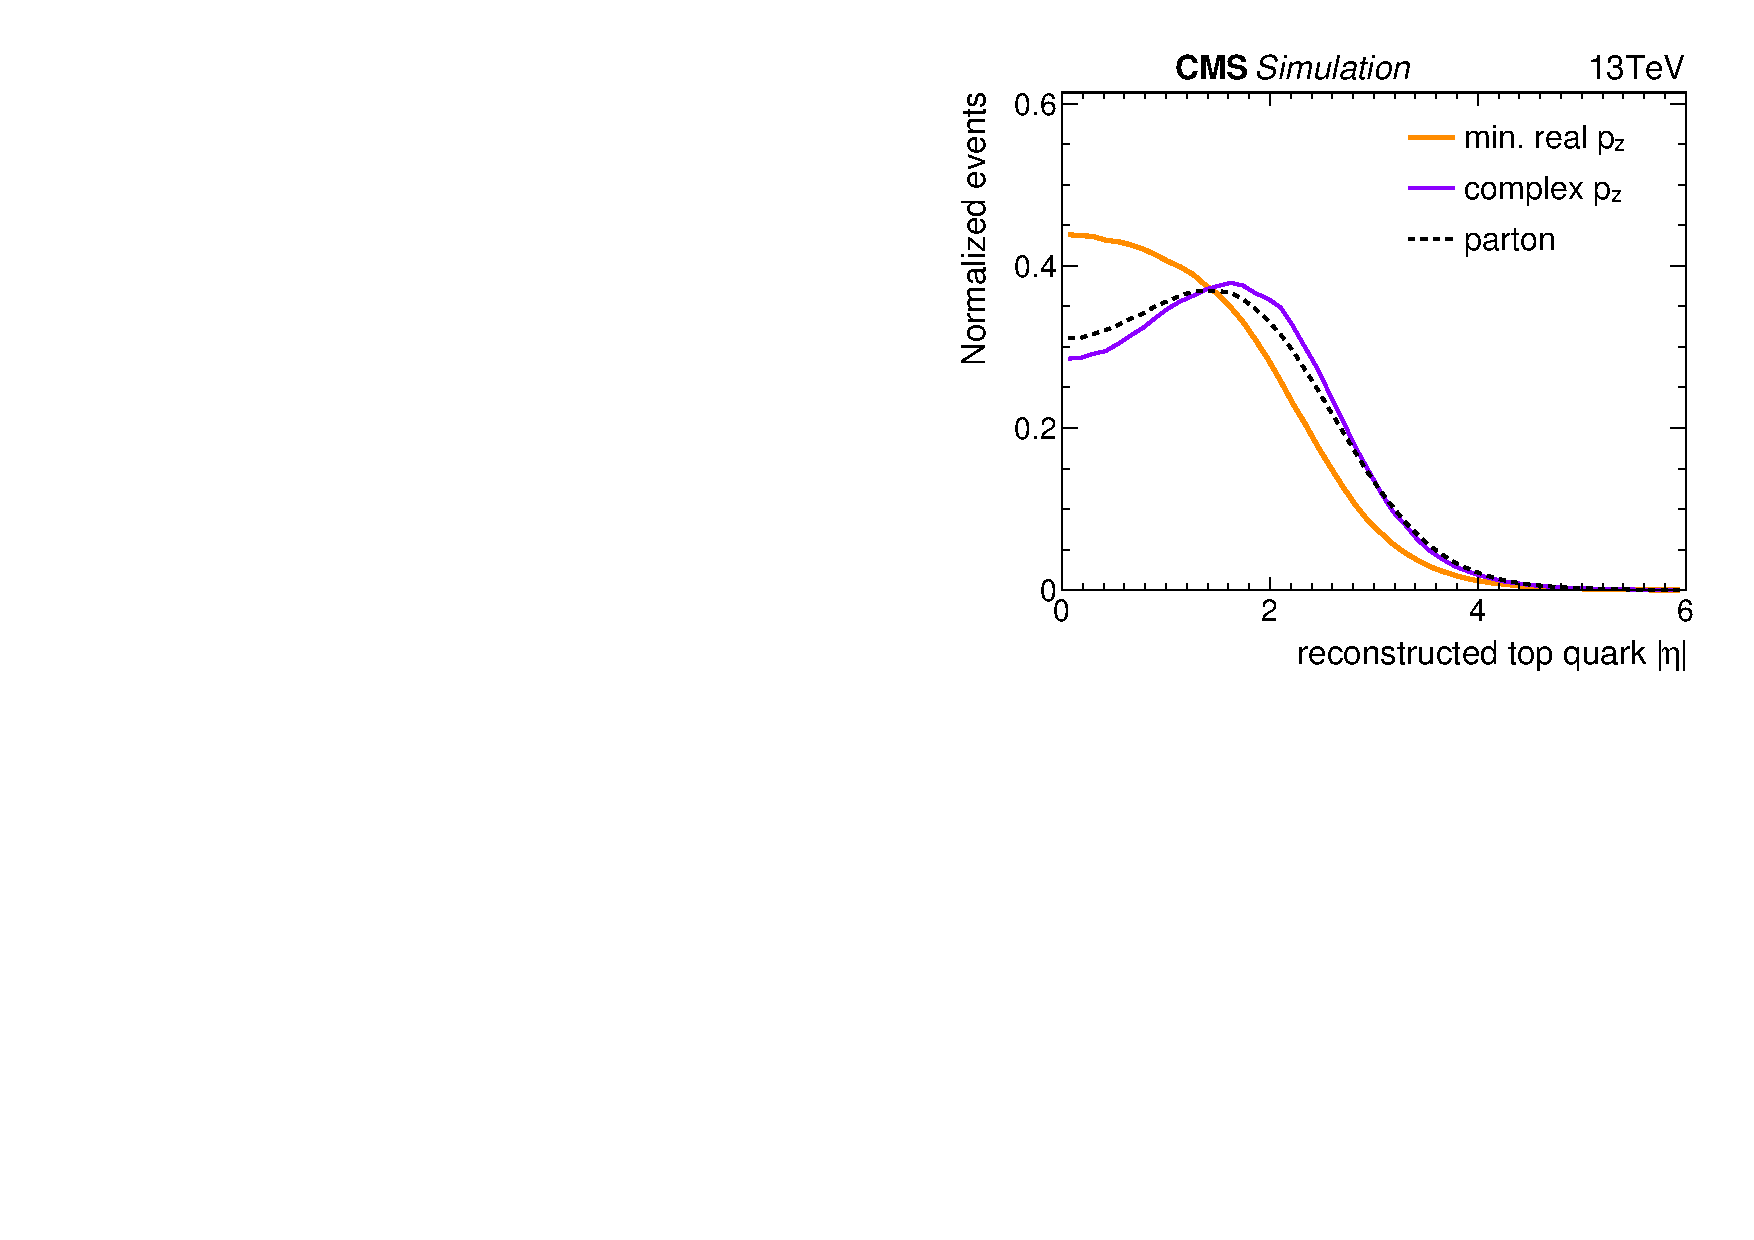
\includegraphics[width=0.48\textwidth]{figures/technique/top_match_eta.pdf}}
}


%##############################################
\section{Boosted Decision Trees}
%##############################################

The $t$-channel single-top-quark signal region, defined by one isolated lepton, 2~jets (where one is b-tagged), and significant \met, is found to be still largely contaminated by events from background processes after the event selection. The \glshere{sb} yield ratios are about 13\% and 14\% in analyses at 8~and 13~TeV, respectively~\cite{Khachatryan:2014iya,Sirunyan:2016cdg}\todo{update TOP-16-003 when accepted by PRL}. The majority of background events stems from \wjets, \ttbar, and multijet production whereas contributions from single top quark tW and $s$-channel, Drell-Yan, and diboson production are minor. The small \gls{sb} ratio motivates the usages \glshere{mva} techniques. In this thesis, \glsplhere{bdt} are employed for event classification as implemented in the \TMVA[] framework~\cite{Hocker:2007ht}. They are based on a set of decision trees where each yields a binary output depending on whether an event is signal- or background-like. Their training and how the single decision tree outputs are combined into a one-dimensional discriminant are detailed in the following.

An exemplary decision tree is presented in Fig.~\ref{fig:technique-decisiontree} where sequential selections on observables $x_{i}$ are applied such that the leaf nodes contain either a majority of signal or background events. Such a tree is build from samples of simulated events for which the desired classification is a priori known~(``superivsed learning'').

\myfigure{\label{fig:technique-decisiontree} A sketch of a decision tree.}{
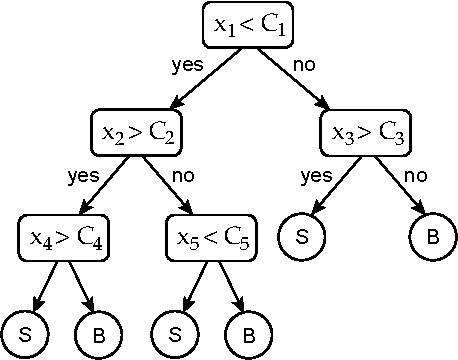
\includegraphics[scale=0.75]{figures/technique/decision_tree.pdf}
}

By maximizing the separation between the signal and background distributions per node the optimal observable $x_{i}$ and working point $C_{i}$  are found. In the analyses, the separation is calculated as the cross entropy 

\begin{align}
H&=-p\cdot\ln(p)-(1-p)\cdot\ln(1-p)\\ p_{i}&=\frac{\int_{C_{i}}^{\infty} N_\mathrm{sig.}(x_{i})\,\mathrm{d}x_{i}}{\int_{C_{i}}^{\infty} N_\mathrm{sig.}(x_{i})+N_\mathrm{bkg.}(x_{i})\,\mathrm{d}x_{i}}\\
\Rightarrow &~\{x_{i},\,C_{i}\}=\max\Big(H\,\big|~x_{i},\,C_{i}\Big)
\end{align}

where $p$ denotes the achieved purity of a selection $x_{i}>C_{i}$. Other common measures of separation are the misclassification error or the so-called ``Gini'' index~\cite{Gini}. The separation measures are constructed to be symmetric when swapping the signal and background classes since obtaining a background leaf with high purity is of equal importance. A node is not split if it contains less than a predefined minimum number of events to ensure that the decisions per node and the binary outputs per leaf are statistically significant. This also mitigates a potential ``overtraining'' of a decision tree which occurs when statistical fluctuations are learned instead of the underlying physical distributions due to the finite statistics of the training sample. Additional caution is required when using a sample which contains a portion of negatively weighted events~(e.g. generated with \MGAMC). In such a case, a tree may be trained incorrectly if a large fraction of negatively weighted events are selected in one of the nodes since the distributions of observables can contain regions with unphysical yields. To tweak the cancellation of negatively weighted events the minimum number of events can be increased further beyond the statistical motivated threshold one would choose when training only on a sample of purely positively weighted events. In addition, the working point values per observable which are analyzed to find the optimal node splitting can be preset which prevents that a decision becomes sensitive to single events close to the selection border.

Single decision trees can still be perceptible to statistical fluctuation leading to misclassification errors when given a statistically-independent test sample. This is mitigated by training multiply decision trees with binary outputs $h_{i}\in\{-1,1\}$ that are then combined into a pseudo-continuous discriminant using a majority vote as

\begin{equation}
M(\vec{x})=\sum_{i}^{N_\mathrm{trees}}~w_{i}\cdot h_{i}\,(\vec{x};\,\vec{C}_{i}).\label{eq:technique-majority-vote}
\end{equation}

Here, each decision tree output is multiplied by a so-called boosting weight $w_{i}$. This way of combining multiple decision trees has another advantage. It has been shown that the majority vote can yield a classifier with high accuracy by applying a ``boosting'' procedure. Such a ``strong learner'' can already be obtained if the individual decision trees are just ``weak learners'' which means that they have only a low classification accuracy~\cite{Schapire1990,FREUND1995256}. The decision trees can therefore be kept very shallow, e.g. only two or three layers of selections, which also improves their robustness against overtraining. A boosting procedure accounts then for the individual accuracy per tree by adjusting its weight accordingly in the majority vote which results into a strong learner.

The two boosting procedures employed in this thesis are the adaptive boosting, \ADABOOST[]~\cite{FREUND1997119}, and \GRADIENTBOOST[]~\cite{Friedman00greedyfunction} algorithms. In the \ADABOOST algorithm, decision trees are trained iteratively. At each step, a single decision tree is trained and the misclassified events are identified. Their weight is then increased in the training of subsequent trees by the boosting weight

\begin{equation}
\alpha_{n+1}=\left(\frac{1-\epsilon_{n}}{\epsilon_{n}}\right)^\beta
\end{equation}

where $\epsilon_{i}$ denotes the misclassification rate of the current tree $n$ and $\beta$ is a configurable learning rate. The corresponding weight in Eq.~\ref{eq:technique-majority-vote} is then given by $w_{i}=\ln\alpha_{i}$. Typically, a slow learning rate of $\beta\leq0.5$ is chosen to allow for more boosting steps. It can be shown that the \ADABOOST algorithm is equivalent to the minimization of the exponential loss function $L(M,y)=\exp(-M(\vec{x})\,y)$ where $y$ denotes the true classification of events~\cite{Hocker:2007ht}. If the loss function is instead changed to 

\begin{equation}
L(M,y)=\ln\left(1+e^{-2\,M(\vec{x})\,y}\right)
\end{equation}

the \GRADIENTBOOST algorithm is obtained. Its loss function is more robust in the presence of outliers and noise events for which the \ADABOOST algorithm may degrade. The algorithm commences by iteratively minimizing the loss function with respect to the weights and decision tree parameters in $M$ using the method of gradient decent. During the minimization steps, the output of the majority vote will gradually tend towards $y$ because misclassified events result in large gradients of the loss function. Similar to the \ADABOOST algorithm, an increased performance is obtained when decreasing the learning rate controlling the boosting weights which is called ``shrinkage'' here. In this thesis, both boosting algorithms have been tested to validate their performances with respect to each other. Only negligible differences in their discrimination power have been found after optimizing their training parameters.

The discrimination power of a trained \gls{bdt} is assessed by analyzing the \glshere{roc} curve. Exemplary \gls{roc} curves are presented in Fig.~\ref{fig:technique-bdt-rocs}. The \gls[]{auc} values denote the area under the \gls{roc} curve with respect to random guessing. Here, the \gls{roc} curves of a \gls{bdt} trained to discriminate $t$-channel single-top-quark events against \wjets and \ttbar background events is compared to the pseudorapidity of the untagged light jet and to the reconstructed top quark mass difference. An \gls{auc} of about $32\%$ is achieved with the trained \gls{bdt} which outperforms the other two typical event observables for separating $t$-channel events from background processes. The exact setup of the \gls{bdt} shown here will be discussed in Sec.~\ref{sec:diff13-bdt} together with the corresponding analysis.

\myfigure{\label{fig:technique-bdt-rocs}Comparison of \gls{roc} curves for separating $t$-channel single-top-quark events from background events (\wjets, \ttbar) using: random guessing; a trained \gls{bdt} discriminant; the pseudorapidity of the untagged light jet ($\jprime$); the difference between the reconstructed top quark mass and the nominal \gls{mc} mass, $|\Delta m_\mathrm{top}|=|m_\mathrm{top}^\scriptn{\mathrm{reco.}}-172.5~\GeV|$.}{
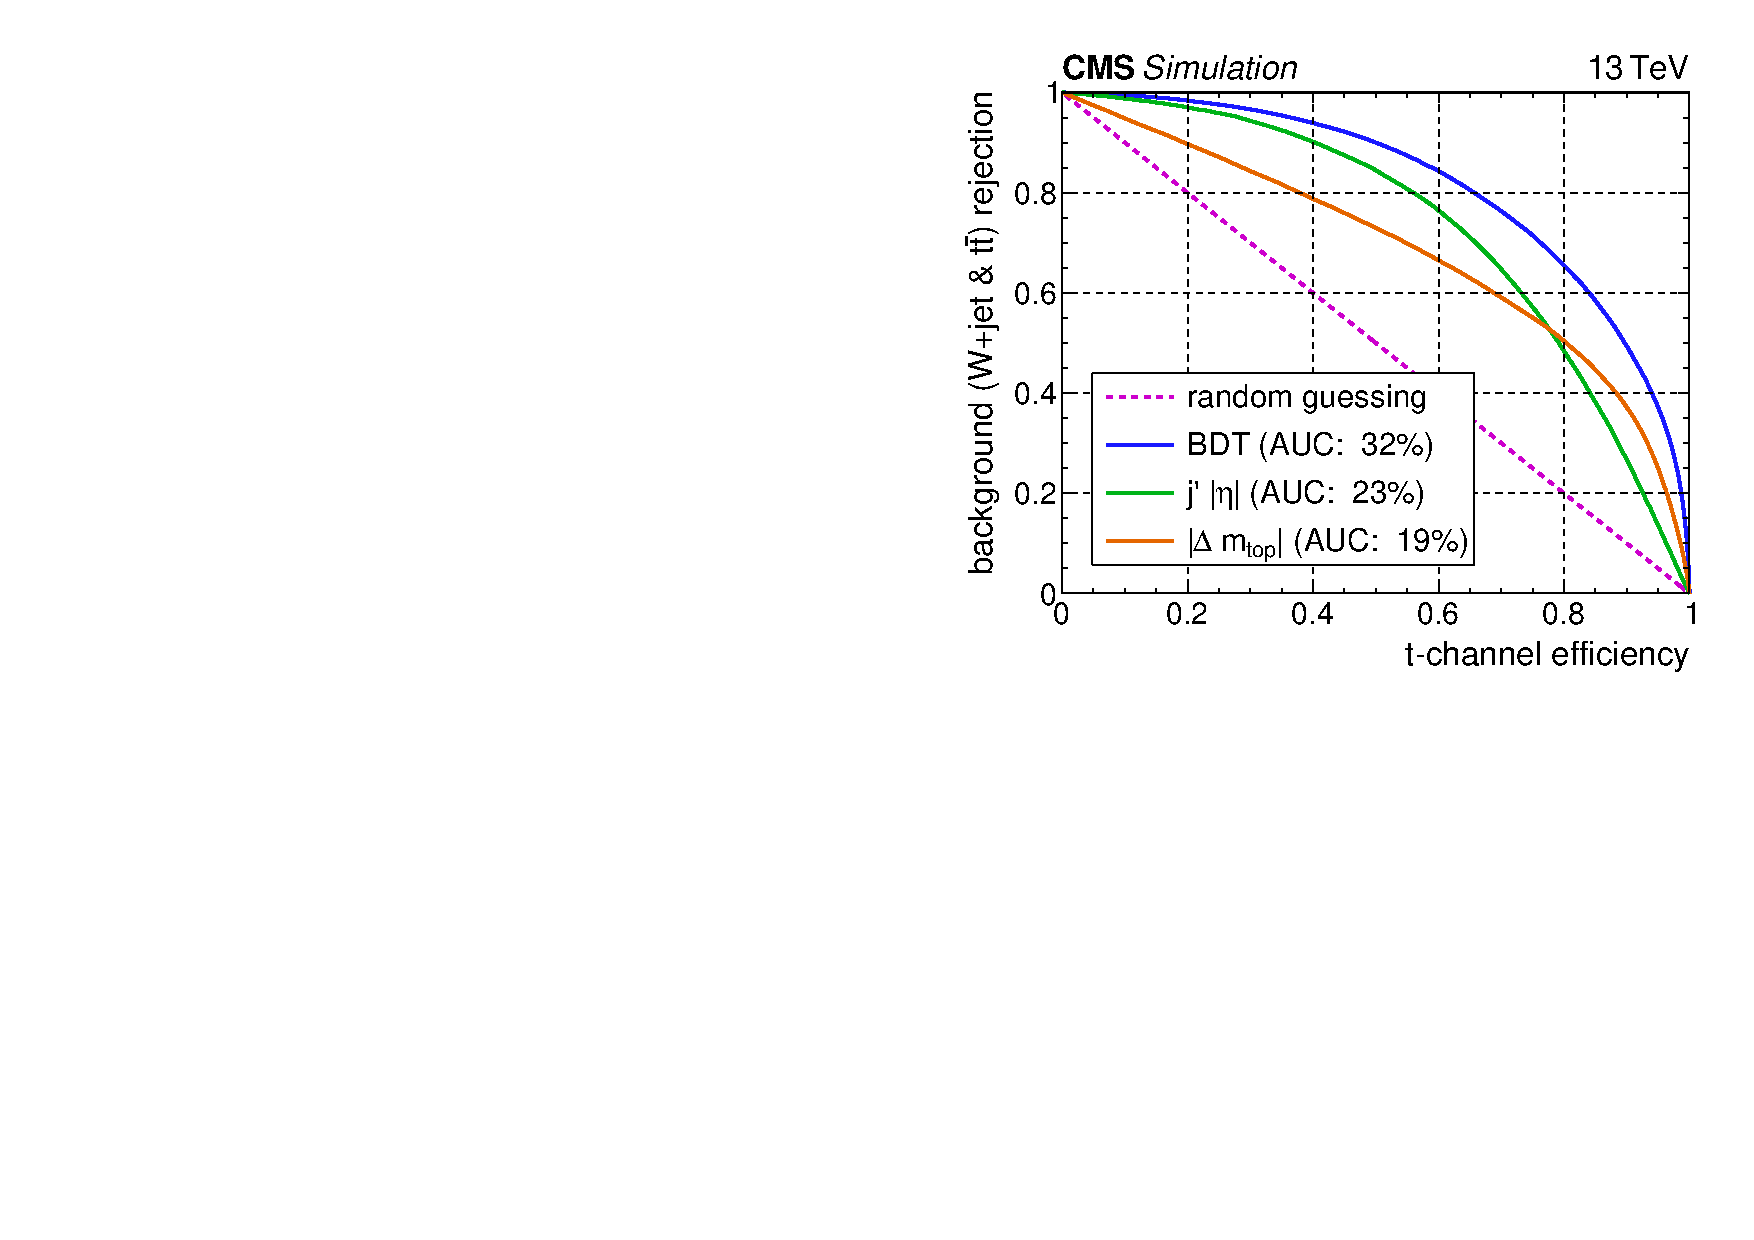
\includegraphics[width=0.5\textwidth]{figures/technique/rocs.pdf}
}


%##############################################
\section{Template-based fitting}
%##############################################

In the analyses, the amount of signal and background events is estimated from data using template-based \glshere{ml} fits. For an observable to be fitted, histograms of simulated events act as templates which reflect the expected distributions of events per process. The likelihood that the observed distribution in data is a realization of the expectation from simulation can then be expressed as

\begin{equation}
\mathsf{L}_\mathrm{Poi.}=\prod_{i}^\mathrm{bins}~\frac{p_{i}^{\,d_{i}}\cdot e^{-p_{i}}}{d_{i}!},\qquad p_{i}=\beta^{\mathrm{(sig.)}}\cdot t^{\mathrm{(sig.)}}_{i}+\sum_{j}^\mathrm{bkgs.}~\beta^{(j)}\cdot t^{(j)}_{i}. \label{eq:technique-likelihood}
\end{equation}

The amount of observed data events $d_{i}$ per bin $i$ is modeled to follow a Poisson distribution with an expected event yield $p_{i}$. The expected yields are obtained by summing the respective contributions of the signal and background templates $t^\scriptn{(X)}_{i}$ per process $X$. The normalization per process is controlled through scale factors $\beta^\scriptn{\mathrm{(X)}}$. These are then estimated through the fit from data by maximizing the likelihood. The signal scale factor is also referred to as signal ``strength'' whereas the background scale factors are sometimes called nuisance parameters because their estimation is of less importance. Technically, the \THETA[] framework~\cite{theta} is employed for template-based fitting where for convenience and numerical stability reasons the negative logarithm of the likelihood

\begin{equation}
-\ln\Big(\mathsf{L}_\mathrm{Poi.}\big(\vec{\beta}\big)\Big)=-\sum_{i}^\mathrm{bins}~\Big[\,d_{i}\ln p_{i}\big(\vec{\beta}\big)-p_{i}\big(\vec{\beta}\big)\Big]+\mathrm{const.}
\end{equation}

is minimized which is however equivalent to maximizing Eq.~\ref{eq:technique-likelihood} with respect to the scale factors. Since the templates are normalized to their corresponding \gls{sm} cross sections times the integrated luminosity, an estimated scale factor can be directly translated into a corresponding cross section as

\begin{align}
\hat{\sigma}_\mathrm{sig.}&=\frac{\hat{N}_\mathrm{sig.}}{A\cdot\epsilon\cdot{\textstyle{\int}L}}~,\quad
\hat{N}_\mathrm{sig.}=\hat{\beta}_\mathrm{sig.}\cdot N_\mathrm{exp.}=\hat{\beta}_\mathrm{sig.}\cdot\underbrace{\sigma_\mathrm{\gls{sm}}\cdot\textstyle{\int}L}_\mathrm{norm.}\cdot \overbrace{A \cdot \epsilon}^\mathrm{sel./reco.}\nonumber\\
&=\hat{\beta}_\mathrm{sig.}\cdot\sigma_\mathrm{\gls{sm}} \label{eq:technique-xsec-measurement}
\end{align}

where $A$ denotes the acceptance and $\epsilon$ the efficiency of the event selection and reconstruction which are intrinsically estimated through the simulated samples. For the background scale factors additional constraints are applied by adding log-normal priors to the likelihood as

\begin{equation}
-\ln\Big(\mathsf{L}_\mathrm{bkgs.}\Big)=\sum_{j}^\mathrm{bkgs.}~\frac{1}{2}\cdot\left(\frac{\ln\,\beta^{(j)}}{\delta^{(j)}}\right)^{2}.
\end{equation}

These additional constraints with uncertainties $\delta$ reflect a priori believes of the background contributions in the signal phase space where the fit is carried out. They are motivated by the fact that the selected analysis phase space is usually only optimized to measure the signal process accurately but not the background contributions. Here, log-normal distributions are explicitly preferred to model the constraints over Gaussian distributions because in the case of large uncertainties log-normal distributions will not be biased when requiring that the scale factors are always positive. For Gaussian distributions with large widths, such a truncation shifts the mean of the distribution which then biases the fit result.

In the fit, an extra uncertainty is considered to account for the limited accuracy of the predicted event yields per bin due to the finite statistics of the simulated event samples. A method proposed by R. Barlow and C. Beeston~\cite{Barlow:1993dm}, commonly called \glshere{bb} method, is to model this uncertainty by adding additional nuisance parameters $\nu_{ij}$ for each bin $i$ and process $j$ which modifies the predicted yields as $p_{i}^\prime=\sum_{j}\nu_{ij}\cdot p_{ij}$. Additional constraints are added to the likelihood which reflect the uncertainties of the sample statistics per parameter. This approach however increases the complexity of the fit since many more parameters have to be estimated in addition to the signal and background scale factors. The number of \gls{bb} parameters is reduced in the Barlow-Beeston lite method~\cite{Conway:2011in} where the uncertainties per bins are grouped and describe by only a single nuisance parameter. A further, technical simplification can be achieved when using numerical minimization algorithms for fitting. Here, it is computationally advantageous to only maximize the likelihood with respect to the scale factors while profiling the \gls{bb} parameters per bin in each step in-situ. This approach is also implemented in the employed \THETA framework. One should note that such an approach can result into discontinuous jumps of the likelihood. Thus, certain minimization algorithms (e.g. \MINUIT~\cite{James:1975dr}) may get confused when the Hessian matrix is found non-positive definite near such discontinuities. Therefore, the simple iterative Newton algorithm is used instead.



%##############################################
\section{Parton and particle level observables}
%##############################################

Cross sections can be measured not only inclusively but also differentially in intervals of an observable. They offer the means to perform in-deep comparisons of data with theoretical predictions. Such measurements allow to assess the modeling and validity of event generators and analytical calculations. Furthermore, as detailed in Ch.~\ref{ch:top}, some differential cross sections can be sensitive to the coupling structure of a process and can thus be used to extract pseudo observables like the top-quark spin asymmetry which is sensitive to the polarization. However, a proper comparison of differential cross sections can only be achieved if the corresponding observable is well-defined and identical across generators and in analytical calculations. There are two ``levels'', parton and particle level, at which physics objects of a process and related observables are typically defined. 

The ``parton level'' encompasses the intermediate and final state particles within Feynman diagrams of a given process while not distinguishing between different initial states. In event generators, these partonic particles are produced as the hard interaction before hadronization. An exemplary event is shown in Fig~\ref{fig:technique-parton-example}. 

\myfigure{\label{fig:technique-parton-example}Production and decay of an exemplary $t$-channel single-top-quark event in 4~\gls{fs} at parton level as produced by \POWHEG{v2} interfaced with \MADSPIN and \PYTHIA{8}. Some intermediate state particles and vertices are not stored by the generator. Copies of particles reflecting the exclusion or inclusion of boosts induced by \gls{qcd}/\gls{qed} radiations have been omitted.}{
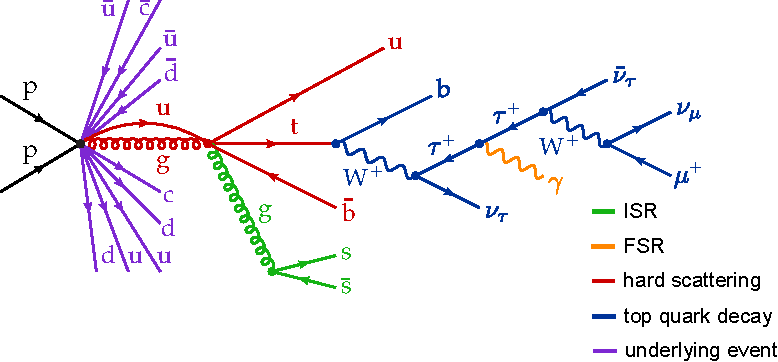
\includegraphics[scale=0.75]{figures/technique/massiveRadiation.pdf}
}

Some intermediate particles and vertices are not stored by the generator for simplicity but also due to the quantum nature of a process. Feyman diagrams corresponds to matrix elements while events are generated to follow the probability of the squared sum of various matrix elements which may also interfere which each other. Therefore, an event cannot be associated with absolute certainty to only one specific Feynman diagram. Nonetheless, various particles and observables can be defined unambiguously at parton level as detailed in the following.
\begin{description}
\item[Prompt leptons] Leptons which originate from decays of Z or W~bosons that are associated to the hard interaction are called ``prompt'' to distinguish them from leptons produced in hadron decays. In $t$-channel single-top-quark production, about 15\% of the prompt muons or electrons originate from the decay of an intermediate tau lepton as exemplary also shown in Fig.~\ref{fig:technique-parton-example}. The fraction depends on the \pt threshold of the muon or electron as depicted in Fig.~\ref{fig:technique-parton-muon}. When selection electron or muons with a $\pt$ of at least $20~\GeV$, this fraction reduces to about 6\%.
\item[Prompt neutrino] Neutrinos are also required to be prompt. In the case of leptonically decaying taus, a prompt ``pseudo'' neutrino is defined by summing the 4-momenta of both neutrinos occurring in the decay.
\item[Top quark] The partonic top quark is defined to be on-shell while accounting for \gls{qcd}/\gls{qed} radiations and the intrinsic \kt of the initial state partons which may boost the event in the transverse plane.
\item[Spectator quark] The spectator quark is required to be produced in association with the single top quark, e.i. they have their ancestors in common as depicted in Fig.~\ref{fig:technique-parton-example}. Furthermore, the spectator quark has be a light flavored quark~(u,d,s,c) to distinguish it from a potential second b~quark occurring in 4~\gls{fs} production. At \gls{nlo}, the production of additional light quarks through \gls{isr} can lead to an ambiguity. In such cases, the quark which balances the transverse top quark momentum is chosen.
\end{description}

\myfigure{\label{fig:technique-parton-muon}Distributions of the (a)~transverse momentum and (b)~pseudorapidity of the final state lepton produced in $t$-channel single top quark production at $13~\TeV$. The lines represent various decays of W~bosons into either muons/taus directly or via intermediate tau decays. The distributions have been generated using \POWHEG{v2} interfaced with \MADSPIN and \PYTHIA{8}.}{
\subfloat[]{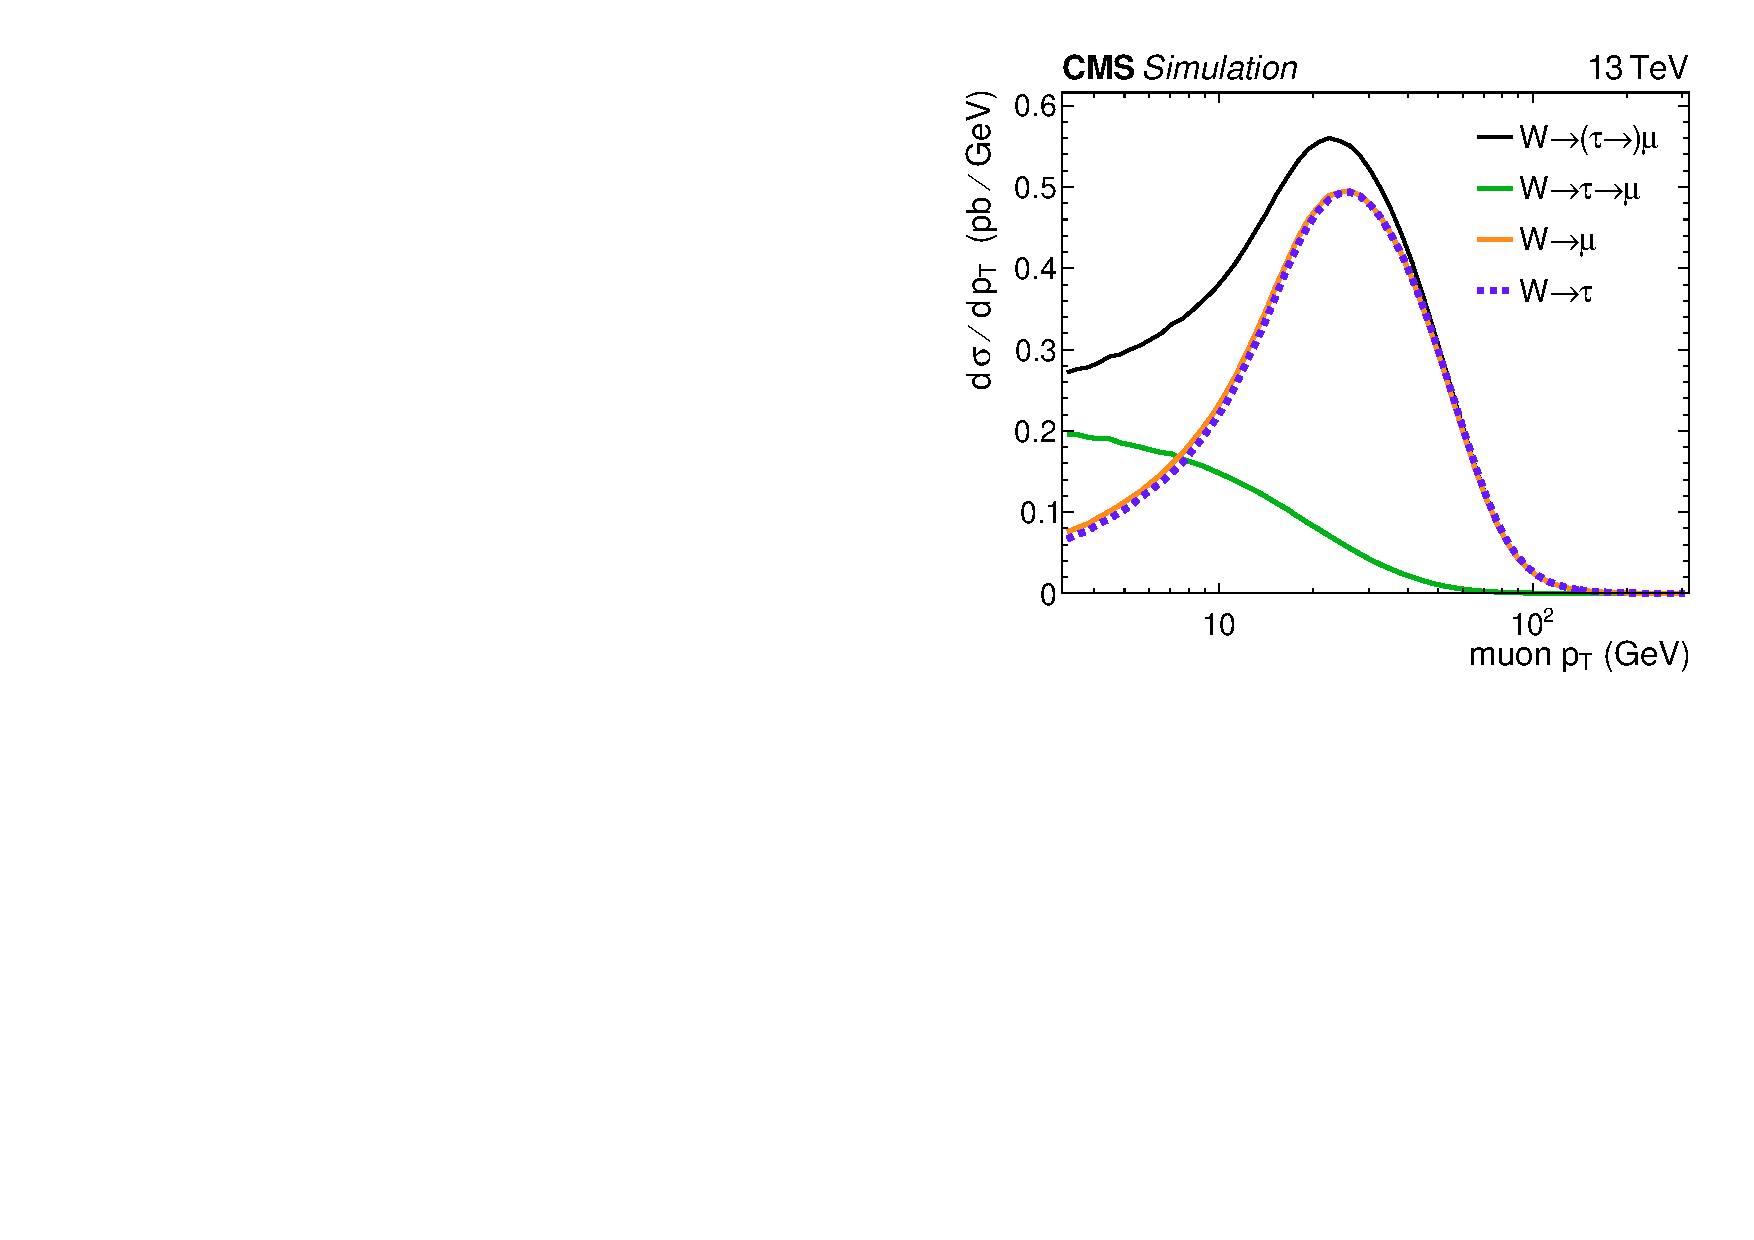
\includegraphics[width=0.48\textwidth]{figures/technique/lepton_pt.pdf}}\hspace{0.03\textwidth}
\subfloat[]{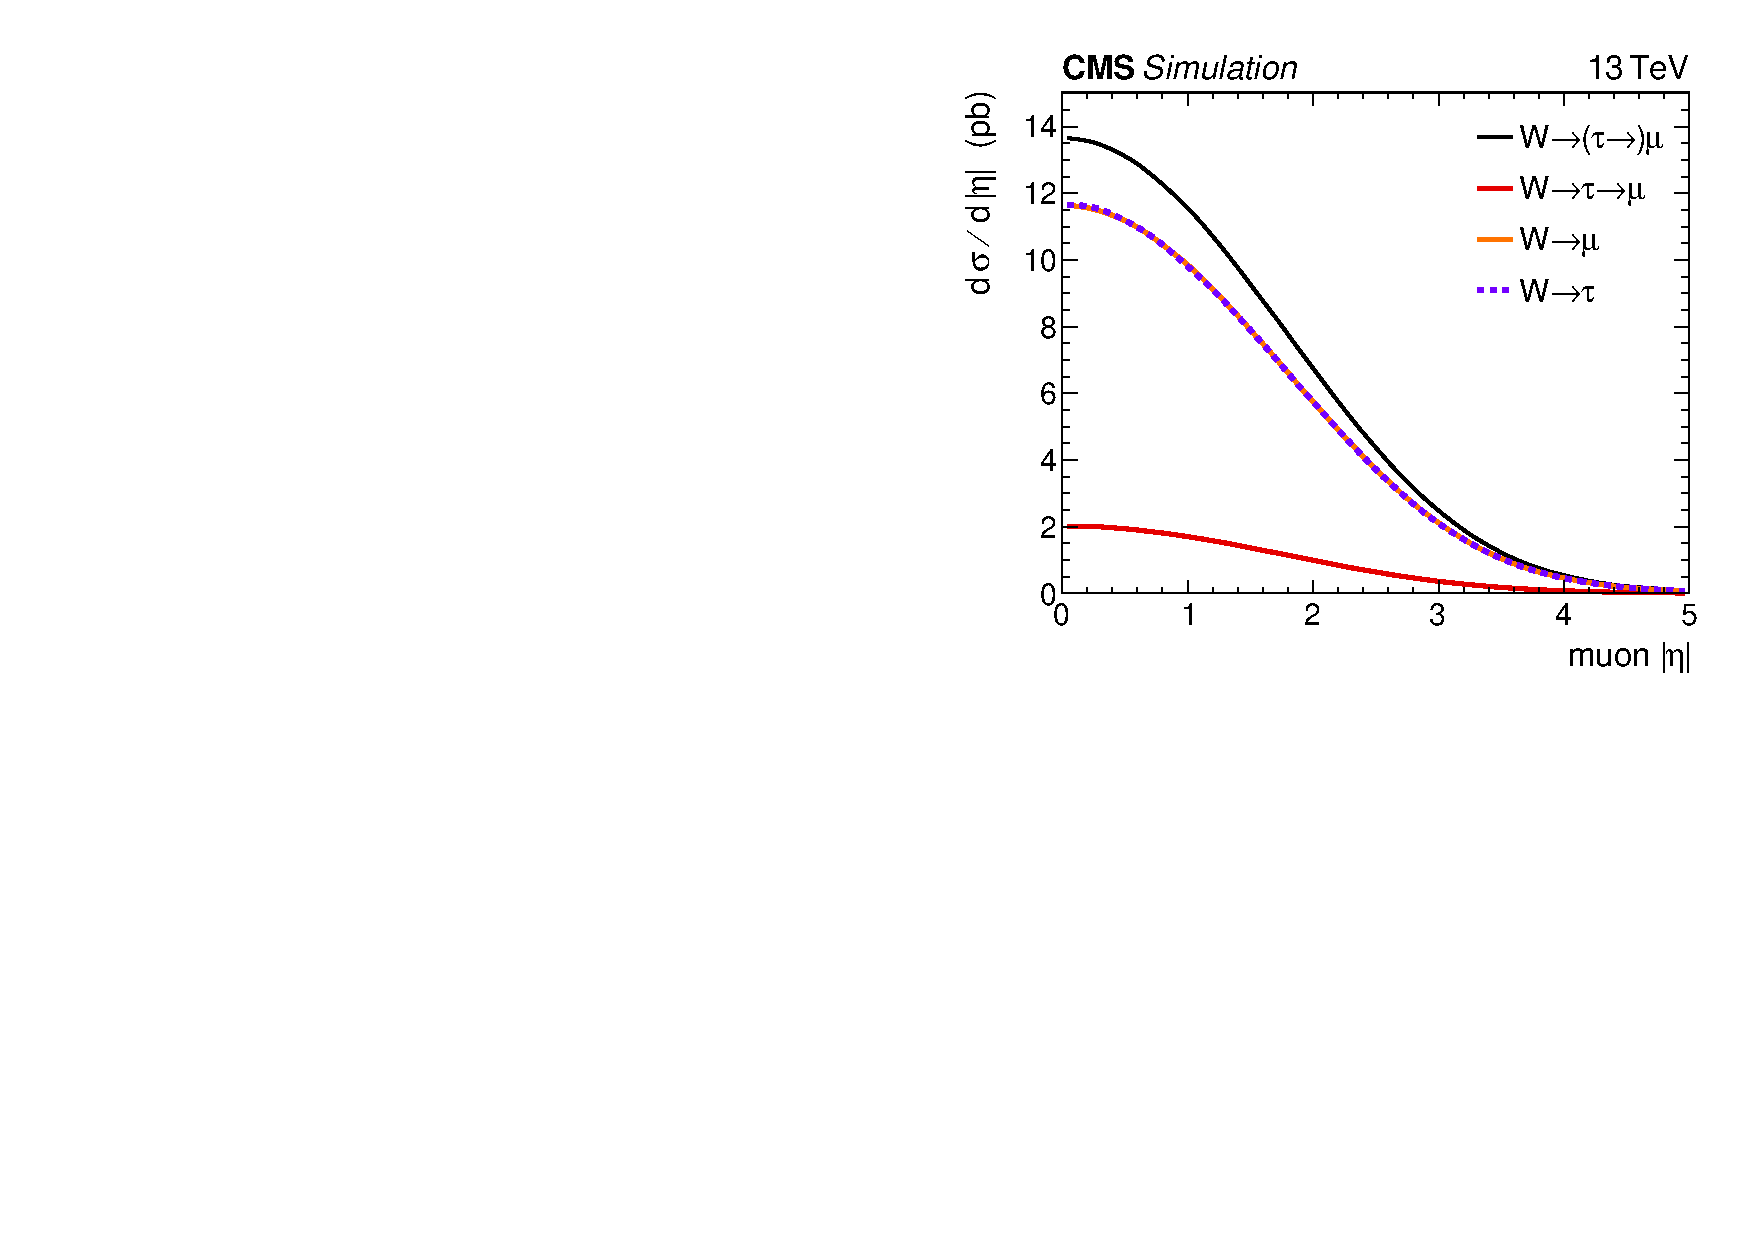
\includegraphics[width=0.48\textwidth]{figures/technique/lepton_eta.pdf}}
}

Using these definitions, the polarization angle can be calculated. A comparison of its shape at parton level for the various lepton decays is presented in Fig.~\ref{fig:technique-parton-cosTheta}. The polarization is nearly identical for tau leptons compared to muons or electrons despite the larger tau mass. \todo{quote asymmetries} The distributions are distorts when requiring a minimum $\pt$ for the prompt lepton which results into a drop of the distribution at $\cos\theta^{*}_{\mu}\to 1$. This is demonstrated in Fig.~\ref{fig:technique-parton-cosTheta20} where the polarization angle is shown for events with $\pt(\mu)>20~\GeV$ only.

\myfigure{\label{fig:technique-parton-cosTheta}Distributions of the polarization angle for $t$-channel single top quark production at $13~\TeV$: (a)~inclusive distribution; (b)~only events with $\pt(\mu)>20~\GeV$. The lines represent various decays of W~bosons into either muons/taus directly or via intermediate tau decays. The distributions have been generated using \POWHEG{v2} interfaced with \MADSPIN and \PYTHIA{8}.}{
\subfloat[]{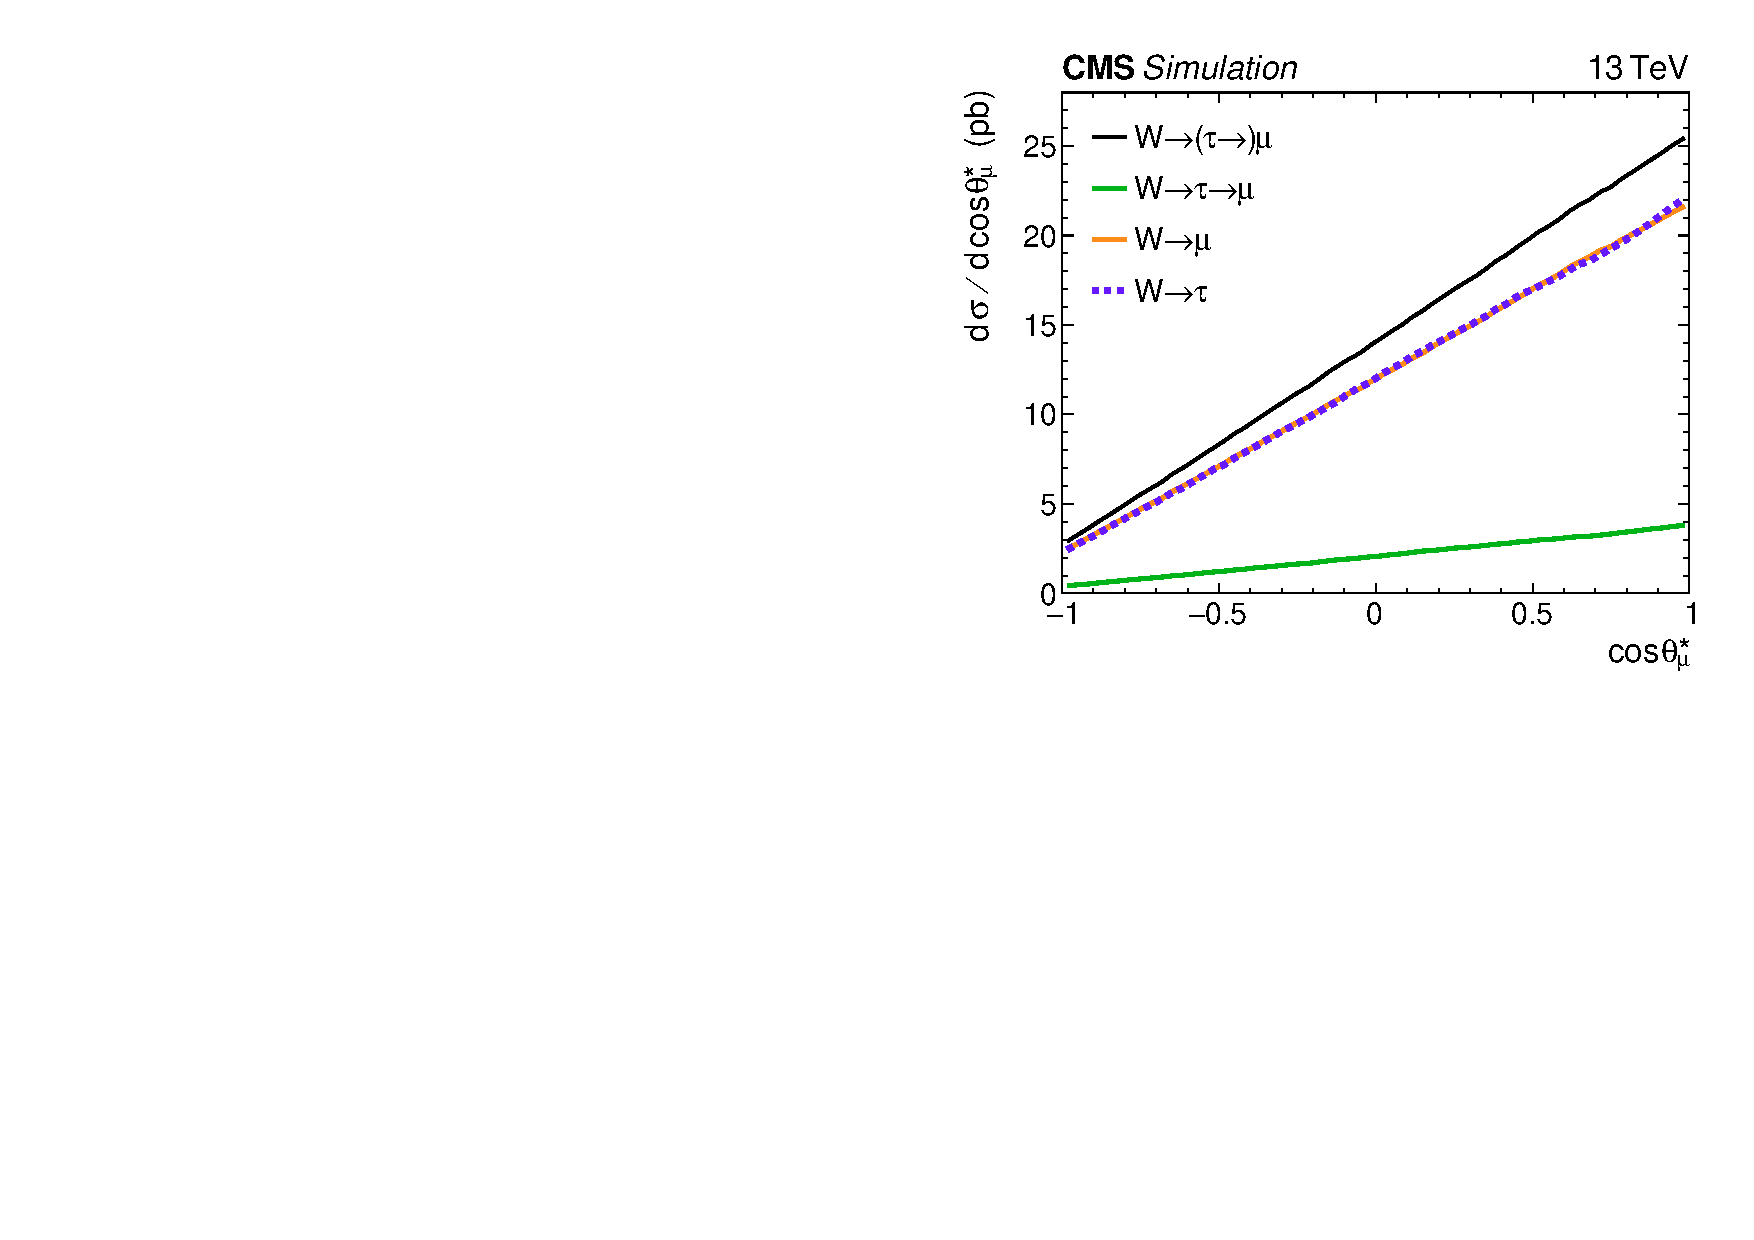
\includegraphics[width=0.48\textwidth]{figures/technique/cosTheta.pdf}}\hspace{0.03\textwidth}
\subfloat[\label{fig:technique-parton-cosTheta20}]{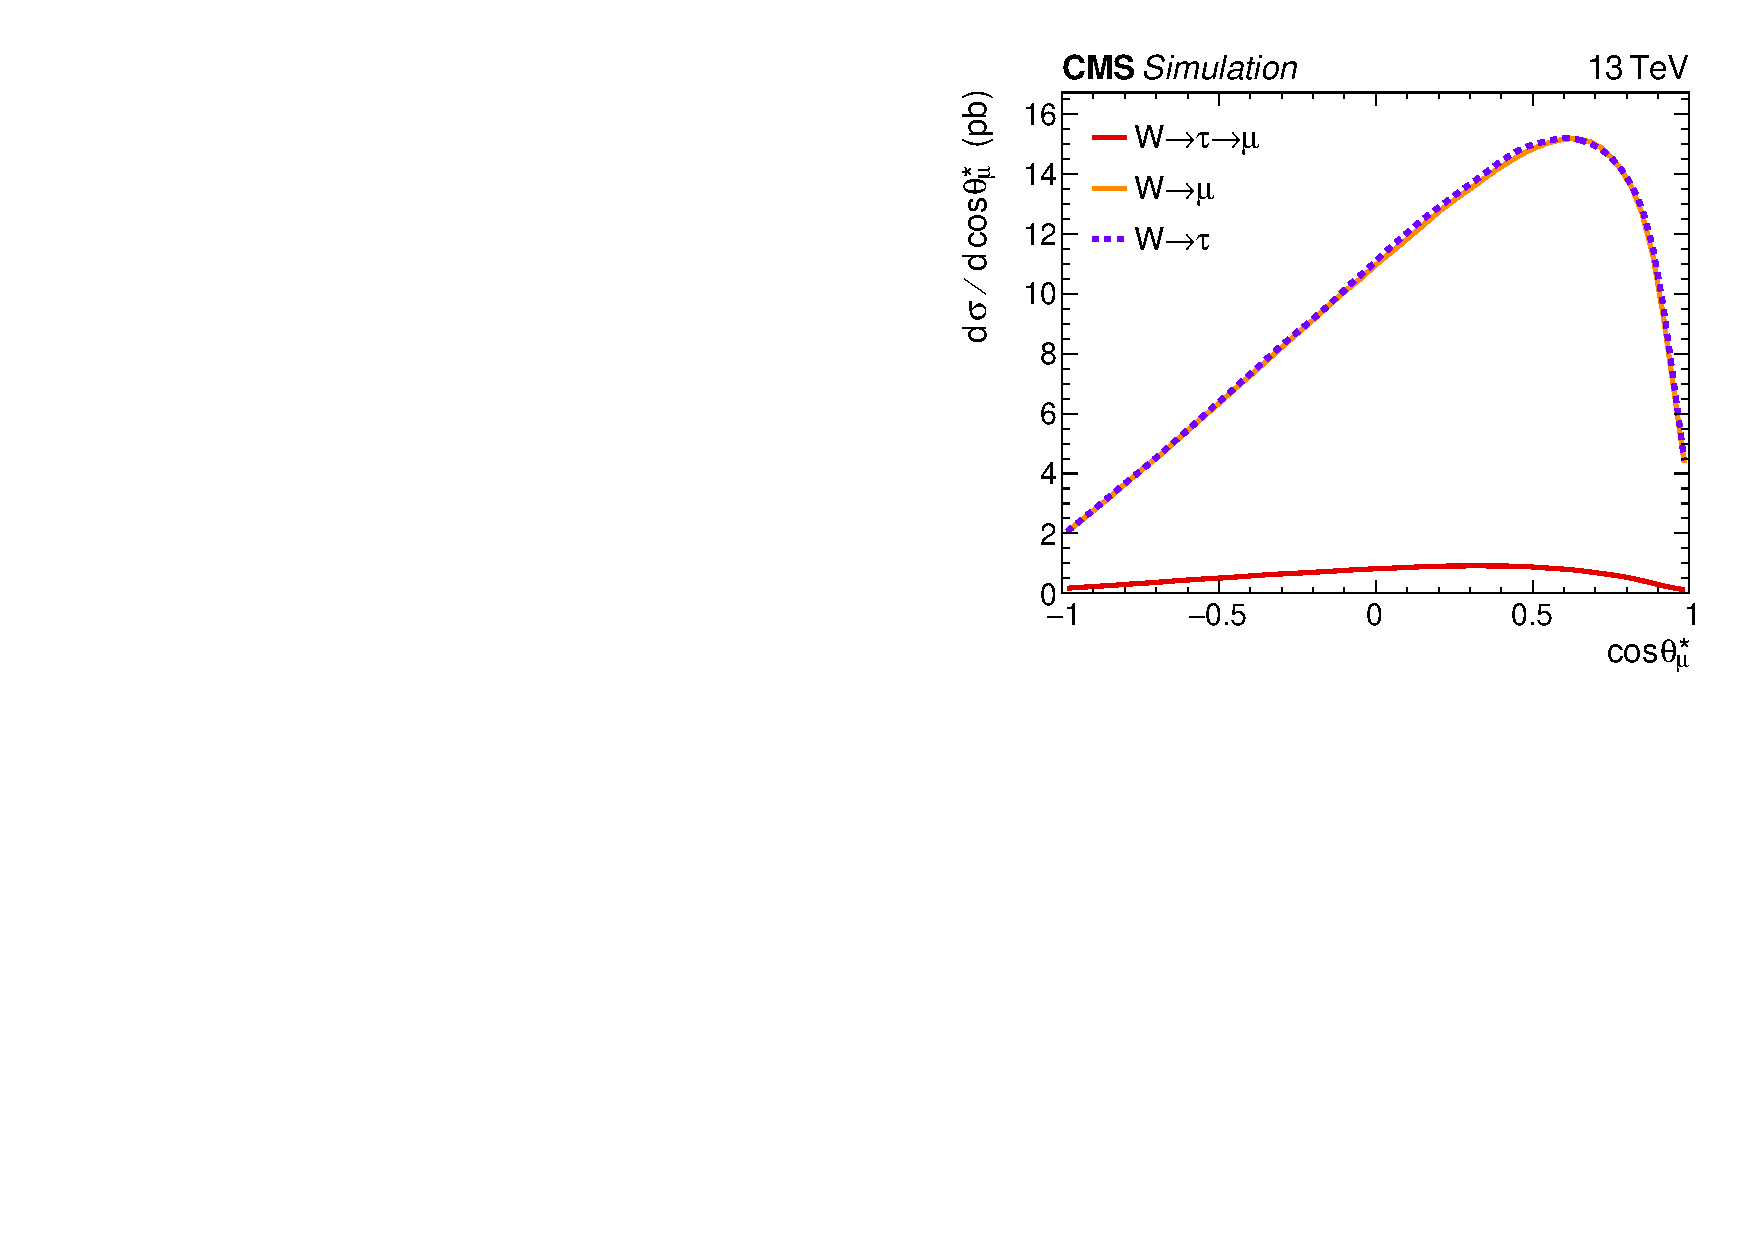
\includegraphics[width=0.48\textwidth]{figures/technique/cosTheta_lpt20.pdf}}
}

The other level at which observables can be defined is the ``particle level''. Here, an event selection similar to the one at reconstruction level is applied on the generated particles after hadronization. This allows to measure a distribution close to the visible phase space of the detector. It is therefore also referred to as ``fiducial'' measurement. The advantage is that an extrapolation into the inclusive phase space as it is intrinsically performed for parton level measurements (e.g. inclusive cross sections) is not required. Furthermore, when defining an observable at parton level, the utilized intermediate particles stored by generators may not follow the same definitions across the various programs. The following statement about the  intermediate particles can be found in the manual of the \RIVET program: ''\textsl{The unfortunate truth is that most of the event record is intended for generator debugging rather than physics interpretation}''~\cite{Buckley:2010ar}. Particle-level observables are on the other hand much less affected by potential implementation-dependent differences. They are defined by utilizing only the final and stable particles produced by event generators and subsequent parton showers with a mean lifetime of more than $30~\mathrm{ps}$.

A comparison of parton and particle level objects for $t$-channel single-top-quark production is shown in Fig.~\ref{fig:technique-parton-particle}. After hadronization, quarks and gluons appear as jets consisting of hadrons and non-prompt leptons at particle level. Charged leptons may radiate photons which are accounted for at particle level by clustering close-by photons with charged leptons. These are referred to as ``dressed'' leptons. The performed clustering enables a universal treatment of \gls{qcd}/\gls{qed} radiations without utilizing information about intermediate particles in the decay chain which is more complicated at parton level (especially in the definition of the spectator quark) and may be generator-dependent as well. Detailed definitions of the analysis objects at particle level used in this thesis are provided in the following.

\myfigure{\label{fig:technique-parton-particle}A sketch of parton and particle level objects in $t$-channel single-top-quark production. An additional gluon has been added as a final state radiation.}{
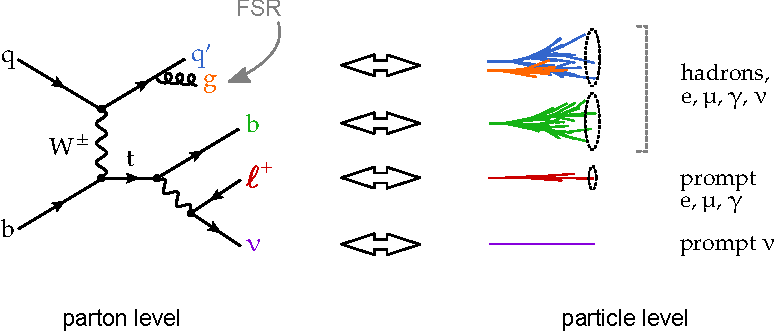
\includegraphics[scale=0.75]{figures/technique/fiducial.pdf}
}

\begin{description}
\item[Dressed leptons] Photons which do not stem from hadron decays are clustered with prompt muons or electrons if they are within $\Delta R=\sqrt{\Delta\eta^2+\Delta\phi^2}<0.1$. A dressed lepton consists of exactly one charged lepton and any number of potential close-by photons.
\item[Neutrinos] The 4-momenta of all prompt neutrinos are summed to define the missing transverse energy. To improve the agreement with the reconstructed neutrino candidate, the same algorithm as described in Sec.~\ref{sec:technique-topreco} is applied at particle level using a dressed lepton here to solve for the neutrino $p_{z}$ component.
\item[Jets] Jet are clustered from stable particles excluding the ones used in the definition of the dressed leptons and all neutrinos. The anti-$k_\mathrm{T}$ algorithm with a distance of $R=0.4$ is employed at 13~TeV mimicking the jet size at reconstruction level. The ``ghost'' b-tagging method~\cite{Cacciari:2008gn} where jet are tagged containing B-hadrons with rescaled momentum will not be used here since its high efficiency disagrees with the performance of the tagging algorithm at reconstruction level~(see Sec.~\ref{sec:diff13-fiducial-studies}).
\item[Pseudo top quark] A pseudo top quark is reconstructed by combining the 4-momenta of a dressed lepton, a neutrino candidate, and a jet.
\end{description}

After applying a suitable selection on the particle level objects, the fiducial cross section can obtained from the inclusive cross section by modifying Eq.~\ref{eq:technique-xsec-measurement} as

\begin{equation}
\sigma_\mathrm{sig.}^\mathrm{fid.}=\frac{N_\mathrm{sig.}\cdot A_\mathrm{fid.}}{A_\mathrm{reco.}\cdot\epsilon_\mathrm{reco.}\cdot{\textstyle{\int}L}} =\sigma_\mathrm{sig.}^\mathrm{inc.}\cdot A_\mathrm{fid.}\,,
\end{equation}

where $A_\mathrm{fid.}$ denotes the acceptance of events. Similar to the acceptance and efficiency of the event selection at reconstruction level, it can be estimated from a sample of simulated signal events as $A_\mathrm{fid.}=N_\mathrm{fid.}/N_\mathrm{total}$. 



%##############################################
\section{Unfolding}
%##############################################

Unfolding in \gls{hep} refers to a procedure which attempts to infer a distribution at parton or particle level from data. In simple terms, the idea of unfolding is to ``revert'' smearing effects, finite resolution, acceptance, and reconstruction inefficiencies of the detector in the recorded data which allows to report a distribution in such a way that it can be easily compared to the expectations from theory and to equivalent measurements, e.g. in other analysis channels or across experiments.

The problem of unfolding can be understood by modeling a reconstructed distribution as 

\begin{equation}
\underbrace{~f(y)~}_\mathrm{reco.}=\int \underbrace{A(y)\,\epsilon(y)\, R(y,x)}_\mathrm{detector}~~\cdot \underbrace{~g(x)~}_\mathrm{true}\, \mathrm{d}x\,, \label{eq:technique-fredholm}
\end{equation}

where a true distribution $g(x)$ (e.i. at parton or particle level) is folded with the detector response $R(y,x)$ times the acceptance of the event selection $A(y)$ and the reconstruction efficiency $\epsilon(y)$. Mathematically, Eq.~\ref{eq:technique-fredholm} is called a Fredholm equation of first kind. Unfolding is then the process to infer the true distribution given $f(y)$, $A(y)$, $\epsilon(y)$, and $R(y,x)$. 

Equation~\ref{eq:technique-fredholm} can be discretized and written as a matrix equation

\begin{equation}
\vec{y} = \widetilde{\mathcal{R}}\cdot\vec{x},\qquad \widetilde{\mathcal{R}}=\mathcal{A}\cdot\mathcal{E}\cdot\mathcal{R}\,, \label{eq:technique-folding}
\end{equation}

where the continuous distributions are converted into vectors~(histograms) and the response, acceptance, and efficiency functions are described by matrices~(two-dimensional histograms). Elements of the response matrix $\mathcal{R}_{ij}$ can be interpreted as the transition probability $p_{i\to j}$ that an event at parton or particle level occurring in bin $i$ is measured in bin $j$. An simple attempt to solve Eq.~\ref{eq:technique-folding} for $\vec{x}$ through a simple inversion of the response matrix reveals that the unfolding problem is actually ill-posed. This results into unstable solutions with large variance and high anticorrelations between bins which can be observed as oscillations~\cite{Cowan:2002in}. Figure~\ref{fig:technique-ill-unfolding} demonstrates this for a simple model defined as

\begin{subequations}
\begin{align}
g(x)&=\frac{1}{2}+A\cdot x\,,\qquad A=0.44\\
R(y,x)&\propto\mathrm{exp}\left(\frac{1}{2}\cdot\frac{(x-y)^2}{\sigma^2}\right)\,,\qquad \sigma=0.15\,,
\end{align}
\label{eq:technique-unfolding-test-model}
\end{subequations}

where a exemplary distribution $g$, similar to the expected distribution of the top-quark polarization angle at parton level, has been folded with a simple Gaussian smearing function $R$. One can observe that small deviations~(dash-orange line) from the folded distribution~(violet markers) yields an unphysical, oscillating solution. Such small deviations may just reflect e.g. statistical fluctuations when unfolding data.

\myfigure{\label{fig:technique-ill-unfolding}Exemplary unfolding of a distribution using a simple inversion of the response matrix: (a)~true distribution with overlaid unfolding results; (b)~the true distribution after folding and a sample of a corresponding statistical fluctuation.}{
\subfloat[\label{fig:technique-ill-unfolding-true}]{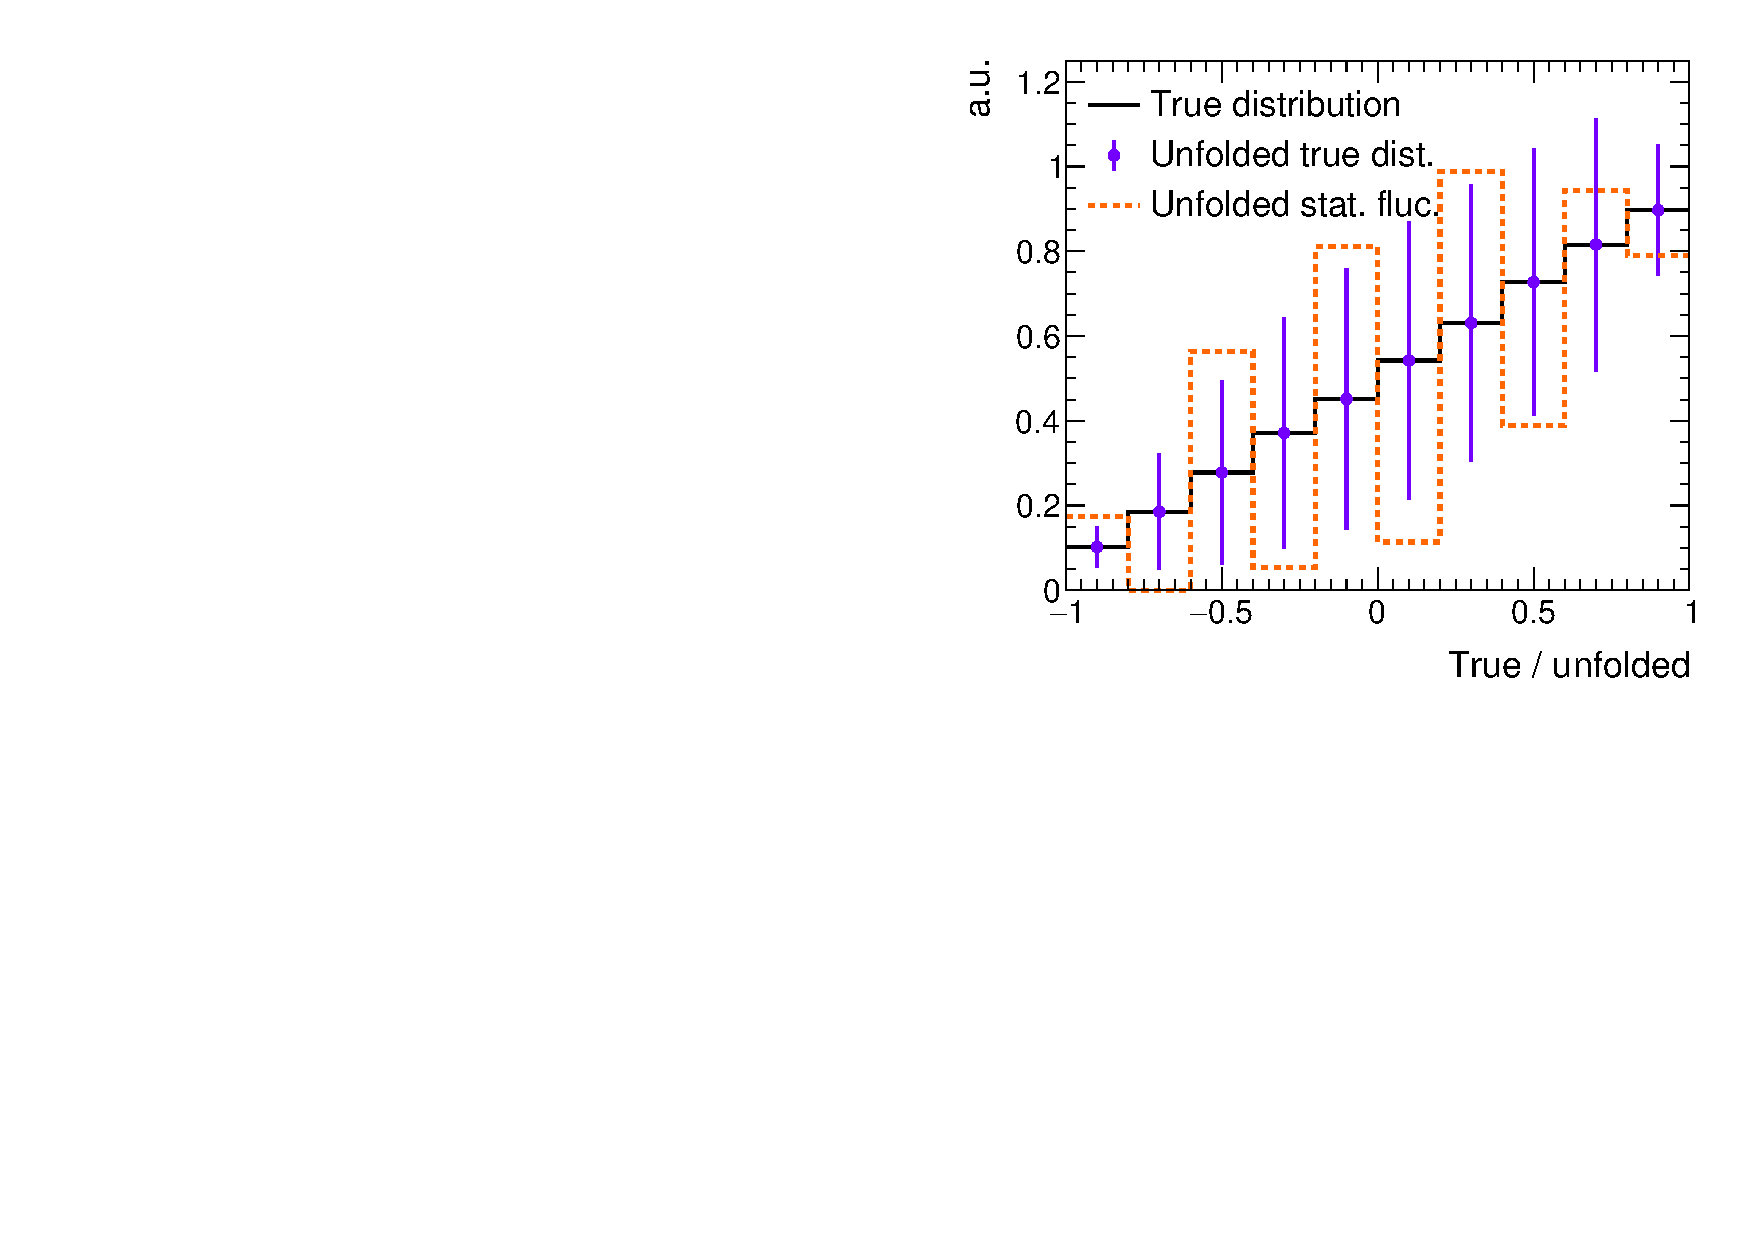
\includegraphics[width=0.48\textwidth]{figures/technique/trueDist.pdf}}\hspace{0.03\textwidth}
\subfloat[\label{fig:technique-ill-unfolding-reco}]{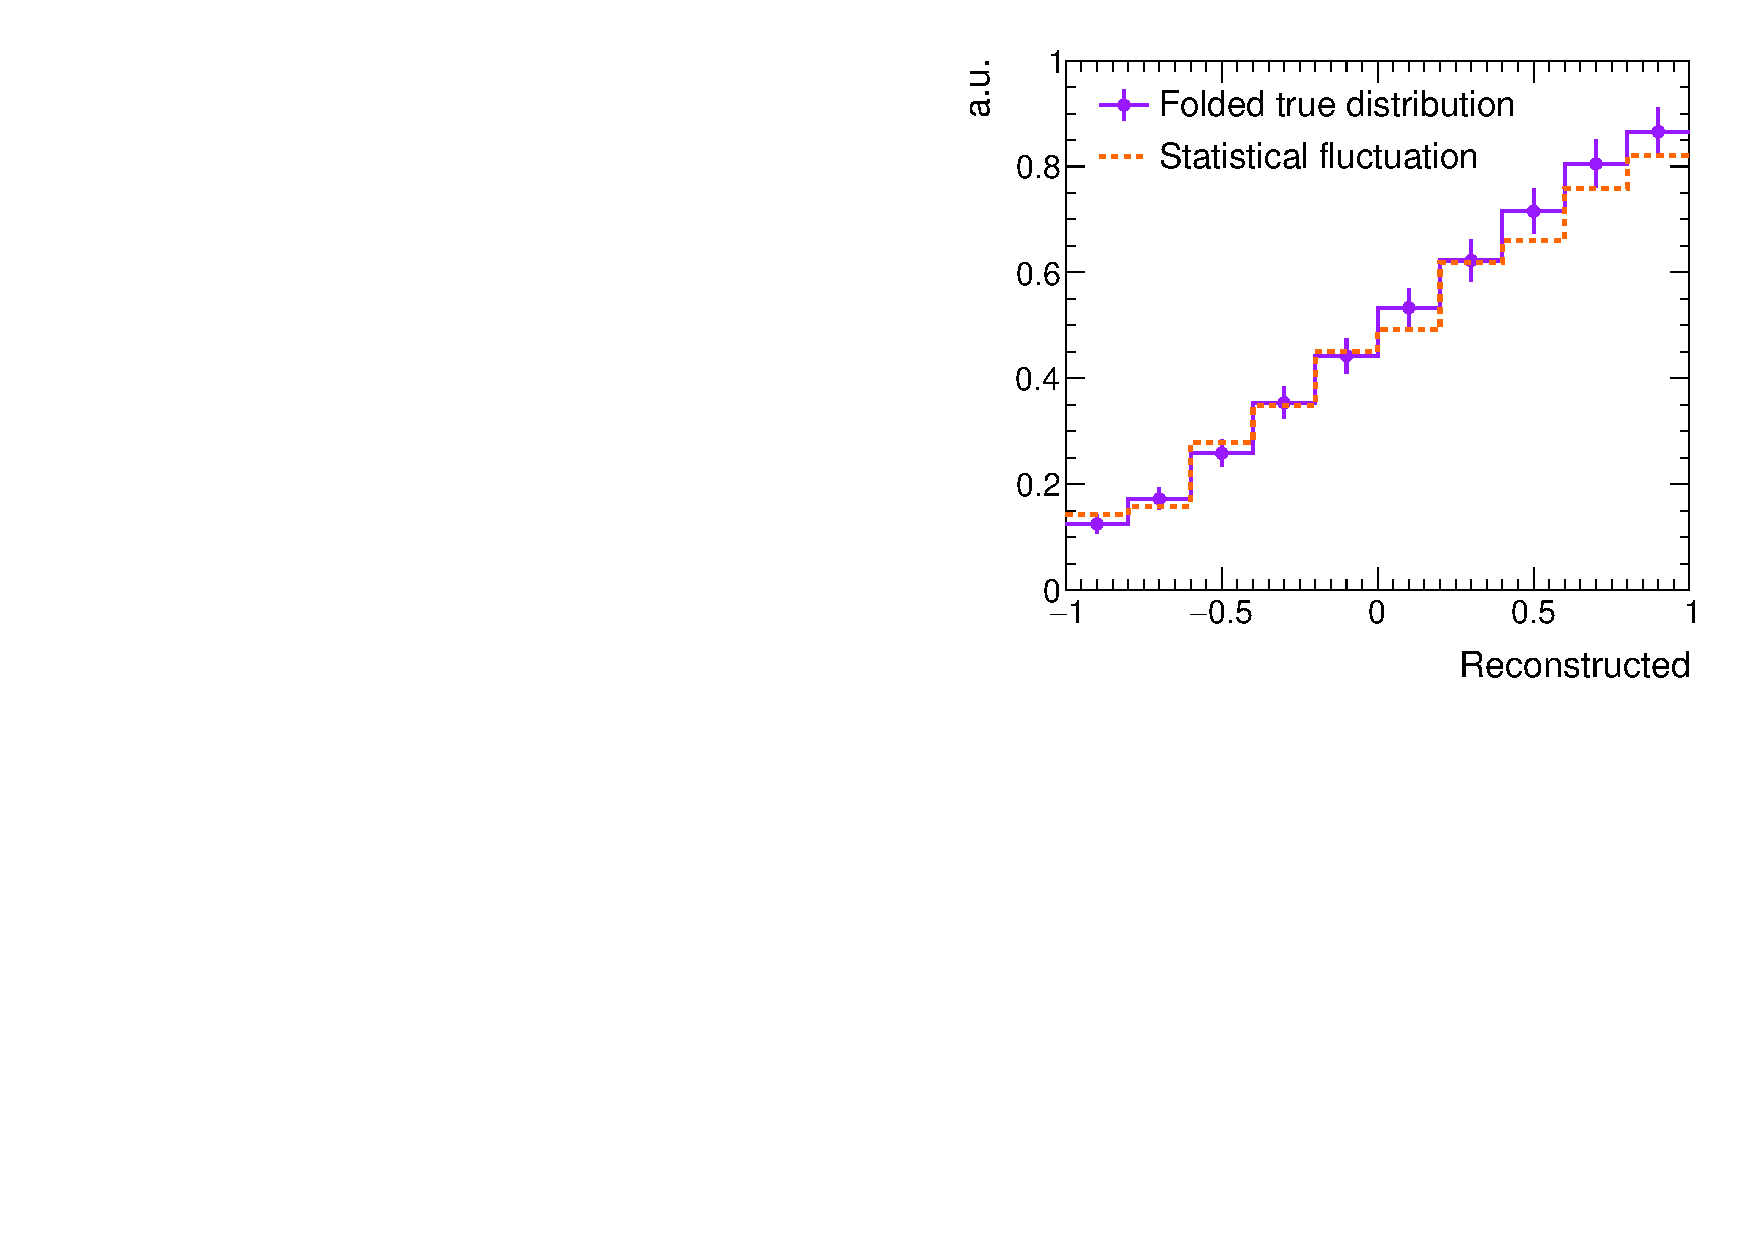
\includegraphics[width=0.48\textwidth]{figures/technique/recoDist.pdf}}
}

This result can be analyzed by performing a \glshere{svd} of the unfolding problem~(Eq.~\ref{eq:technique-folding}). \Gls{svd} is a generalization of the eigendecomposition that allows to decompose even non-quadratic matrices into 

\begin{equation}
\vec{x}=\Big(\widetilde{\mathcal{R}}\Big)^{-1}\vec{y}\\
=\Big(\mathcal{U}~\cdot\underbrace{\mathcal{S}}_\mathrm{diagonal}\cdot~\mathcal{V}\Big)^{-1}\vec{y}~=~\mathcal{V}^{-1}\cdot
\begin{tikzpicture}[baseline=(current bounding box.center),every left delimiter/.style={xshift=0.4em},every right delimiter/.style={xshift=-.4em},]
\matrix (m) [matrix of math nodes,nodes in empty cells,row sep=-1.5mm,left delimiter=(,right delimiter={)},inner sep=0pt,nodes={inner sep=.3333em},]{
\frac{1}{s_{11}} &  & 0  \\
0 & & \frac{1}{s_{nn}} \\
} ;
\draw[dotted,thick] (m-1-1)-- (m-2-3);
\end{tikzpicture}
\cdot~~\mathcal{U}^{-1}~\vec{y}\,,
\end{equation}


where $\mathcal{U}$ and $\mathcal{V}$ contain the so-called left- and right-singular vectors, respectively. The matrix $\mathcal{S}$ has only non-zero elements $s_{ii}$ on its diagonal which are also referred to as singular values. Typically, they are ordered as $s_{ii}>s_{i+1,i+1}$ while the singular vectors are normalized to $1$. The vectors are orthogonal to each other and can be interpreted as modes of the measured distribution. When a singular value is small, the unfolded distribution becomes unstable since the corresponding mode in the reconstructed distribution is unphysically amplified by $1/s_{ii}$ through the inversion.

Various regularization procedures have been proposed to mitigate this problem. The most straight forward regularization scheme is utilized in the ``\gls{svd} unfolding'' algorithm~\cite{Hocker:1995kb}. It modifies the response matrix as

\begin{equation}
\Big(\mathcal{R}^\mathrm{reg.}[\tau]\Big)^{-1}_{ ij}=\sum_{i}^{n}\,\left(\,\sum_{k}^{\tau}~\mathcal{V}^{-1}_{ik}\cdot\left(\frac{1}{s_{kk}}\right)\cdot~\mathcal{U}^{-1}_{kj}\right)\,,
\end{equation}

where the regularization parameter $\tau$ controls a cutoff that keeps only singular values with indices $k\leq\tau<n$ during the inversion. Thus, higher order modes in the reconstructed distribution leading to oscillating solutions are ignored. A more sophisticated unfolding method is the Tikhonov regularization scheme~\cite{Tikhonov}. It rewrites the unfolding problem as a minimization of the loss function

\begin{align}
L\big(\vec{x}\big)&=\big|\big|\,\vec{y}-\tilde{\mathcal{R}}\cdot\vec{x} \,\big|\big|^{2}~+~~\big|\big|\,\Gamma\cdot\vec{x}\,\big|\big|^{2}\qquad\Rightarrow~~\frac{\partial L}{\partial x_{i}}=0\,,
\end{align}

where a suitable matrix $\Gamma$ is added to suppress unphysical solutions. In this thesis, unfolding is performed using the \TUNFOLD[] package~\cite{1748-0221-7-10-T10003} which employs a similar regularization scheme. Its loss function is given by

\begin{subequations}
\begin{align}
L_\mathrm{\TUNFOLD}\big(\,\vec{x},\,\lambda\,\big|~\tau\big)&=\sum_{i}\,\sum_{j}~\Big(y_{i}-\big(\tilde{\mathcal{R}}\cdot\vec{x}\,\big)_{i}\Big)\cdot\mathcal{C}_{y,ij}^{-1}\cdot\Big(y_{j}-\big(\tilde{\mathcal{R}}\cdot\vec{x}\,\big)_{j}\Big)\label{eq:technique-tunfold-response}\\
&+\tau^{2}\cdot\Big(\Gamma\cdot\big(\vec{x}-\vec{x}_{0}\big)\Big)^{2}\label{eq:technique-tunfold-regularization}\\
&+\lambda\cdot\sum_{i}~\Big(y_{i}-\mathcal{A}_{ii}\mathcal{E}_{ii}x_{i}\Big)\,. \label{eq:technique-tunfold-efficiency}
\end{align}
\label{eq:technique-tunfold}
\end{subequations}

The matrix $\mathcal{C}$ in Eq.~\ref{eq:technique-tunfold-response} describes the statistical covariances of the bins in the reconstructed distribution. For uncorrelated data bins it is a diagonal matrix with entries $\mathcal{C}_{ii}=y_{ii}$ assuming Poisson uncertainties. Regularization is applied through the penalty term in Eq.~\ref{eq:technique-tunfold-regularization}. Here, solutions with large fluctuations are suppressed through the matrix $\Gamma$ which approximates numerically the second derivatives per bin of the resulting distribution as 

\begin{equation}
\frac{\mathrm{d}^{2}g(x)}{\mathrm{d}x^2}\approx\frac{g(x-h)-2\,g(x)+g(x+h)}{h^2}\,,~~\Rightarrow~\Gamma=
\begin{tikzpicture}[baseline=(current bounding box.center),every left delimiter/.style={xshift=1.1em},every right delimiter/.style={xshift=-0.3em}]
\matrix (m) [matrix of math nodes,nodes in empty cells,left delimiter=(,right delimiter={)},inner sep=0pt,nodes={inner sep=.3333em},]{
\hphantom{-}1 & -2            & \hphantom{-}1 & \hphantom{-}0 & \hphantom{-}0\\
\hphantom{-}0 & \hphantom{-}1 & -2            & \hphantom{-}1 & \hphantom{-}0  \\
              &               &               &               &   \\[0.5em]
\hphantom{-}0 & \hphantom{-}0 & \hphantom{-}1 & -2            & \hphantom{-}1 \\
} ;
\draw[dotted,thick] (m-2-2)-- +(0.65,-0.6);
\draw[dotted,thick] (m-2-1)-- +(0.65,-0.6);
\draw[dotted,thick] (m-2-3)-- +(0.65,-0.6);
\draw[dotted,thick] (m-2-4)-- +(0.65,-0.6);
\end{tikzpicture}\,.~
\end{equation}

The regularization strength is controlled with the parameter $\tau$ and needs to be optimized as detailed below. The vector $\vec{x}_{0}$ allows to bias the calculation of the second derivatives. It is usually set to the expectation from theory. This way, the regularization vanishes when unfolding the expectation from theory for closure tests since $(\Gamma\,(\vec{x}_\mathrm{exp.}-\vec{x}_{0}))^2=0$. Thus, the result is bias-free even for heavily curved expectations like e.g. $\pt$ spectra of particles. An alternative procedure to achieve this is to reweight $\vec{y}$ such that $x_{i}^\prime=x_{i}/x_{i}^\scriptn{\mathrm{exp.}}$ which lets the regularization vanish as well when unfolding the expectation since $\Gamma\,\vec{x}^{\,\prime}_\mathrm{exp.}=0$. The last part of the loss function, Eq.~\ref{eq:technique-tunfold-efficiency}, attempts to match the overall normalization of the solution by accounting for the acceptance and reconstruction efficiencies per bin. It is minimized independently with respect to the Lagrange parameter $\lambda$.

Finding the optimal regularization strength is of crucial importance. If the applied regularization is too weak, the unfolding with become unregulated and thus leads to unphysical solutions with oscillating behavior. On the other hand, if the regularization is too strong, the solution will be biased towards the solution of minimum curvature. Here, the solution might tend towards the expectation from theory since either through the application of a bias vector or the described reweighting, it is one solution with vanishing curvature. A method to analyze the unfolding behavior is to monitor the induced bin-by-bin correlations as a function of the regularization strength. The covariance matrix of the unfolded spectrum is given by propagation of uncertainty as

\begin{equation}
\mathcal{C}_{x}[\tau]=J\cdot\mathcal{C}_{y}\cdot J^{T}=\tilde{\mathcal{R}}^{-1}_\mathrm{reg.}[\tau]\cdot\mathcal{C}_{y}\cdot\big(\tilde{\mathcal{R}}^{-1}_\mathrm{reg.}[\tau]\big)^{T}\,,
\end{equation}

where $J$ denotes the Jacobian matrix which is equal to the regularized and inverted response matrix as obtained through the minimization of Eq.~\ref{eq:technique-tunfold}. This allows to define the average correlation between bins as

\begin{equation}
\bar{\rho}_{j}[\tau]\equiv\frac{1}{n-j-1}\sum_{i}^{n-j-1}\rho_{i,i+j}[\tau],\qquad \rho_{i,j}[\tau]=\frac{\mathcal{C}_{x,ij}[\tau]}{\sqrt{\mathcal{C}_{x,ii}[\tau]\cdot\mathcal{C}_{x,jj}[\tau]}}\,.\label{eq:technique-avg-correlation}
\end{equation}

Figure~\ref{fig:technique-tauscan-scan} presents the averaged correlations as a function of the regularization strength for the model defined in Eq.~\ref{eq:technique-unfolding-test-model}. This so-called ``subway plot''\footnote{Such plots have been developed in my Master's thesis~\cite{Komm-thesis}.} visualizes the three different regions of solution classes. The first regions on the left contains solutions where $\bar{\rho}_{1}<0$ thus indicating large anticorrelations between directly adjacent bins which can be observed as an oscillation as demonstrated in Fig.~\ref{fig:technique-ill-unfolding-true}. On the right side where $\bar{\rho}_{1}>0$ the solutions are found biased towards a solution with minimal curvature. In intermediate region solutions with vanishing the correlations can found which however do not occur at the same regularization strength. Here, the average global correlation which is calculated as

\begin{equation}
\rho^\mathrm{global}_{ i}[\tau]=\sqrt{1-\frac{1}{\mathcal{C}_{x,ii}[\tau]\cdot\big(\mathcal{C}_{x}^{-1}[\tau]\big)_{ii}}}\,,\label{eq:technique-global-correlation}
\end{equation}

provides a suitable trade-off as indicated by the black solid curve for choosing a regularization strength with minimal correlations across the unfolded spectrum. The resulting regularized unfolding result is shown in Fig.~\ref{fig:technique-tauscan-result} which does not exhibit the oscillating behavior as shown in Fig.~\ref{fig:technique-ill-unfolding-true}. Furthermore, regularization has stabilized the result against small deviations as indicated by the reduced variances.

\myfigure{\label{fig:technique-tauscan}Regularized unfolding using the \TUNFOLD package: (a)~the average bin-by-bin correlations~(Eqs.~\ref{eq:technique-avg-correlation} and~\ref{eq:technique-global-correlation}) as a function of the regularization strength; (b)~the resulting spectrum when choosing the regularization at the minimum of the averaged global correlation.}{
\subfloat[\label{fig:technique-tauscan-scan}]{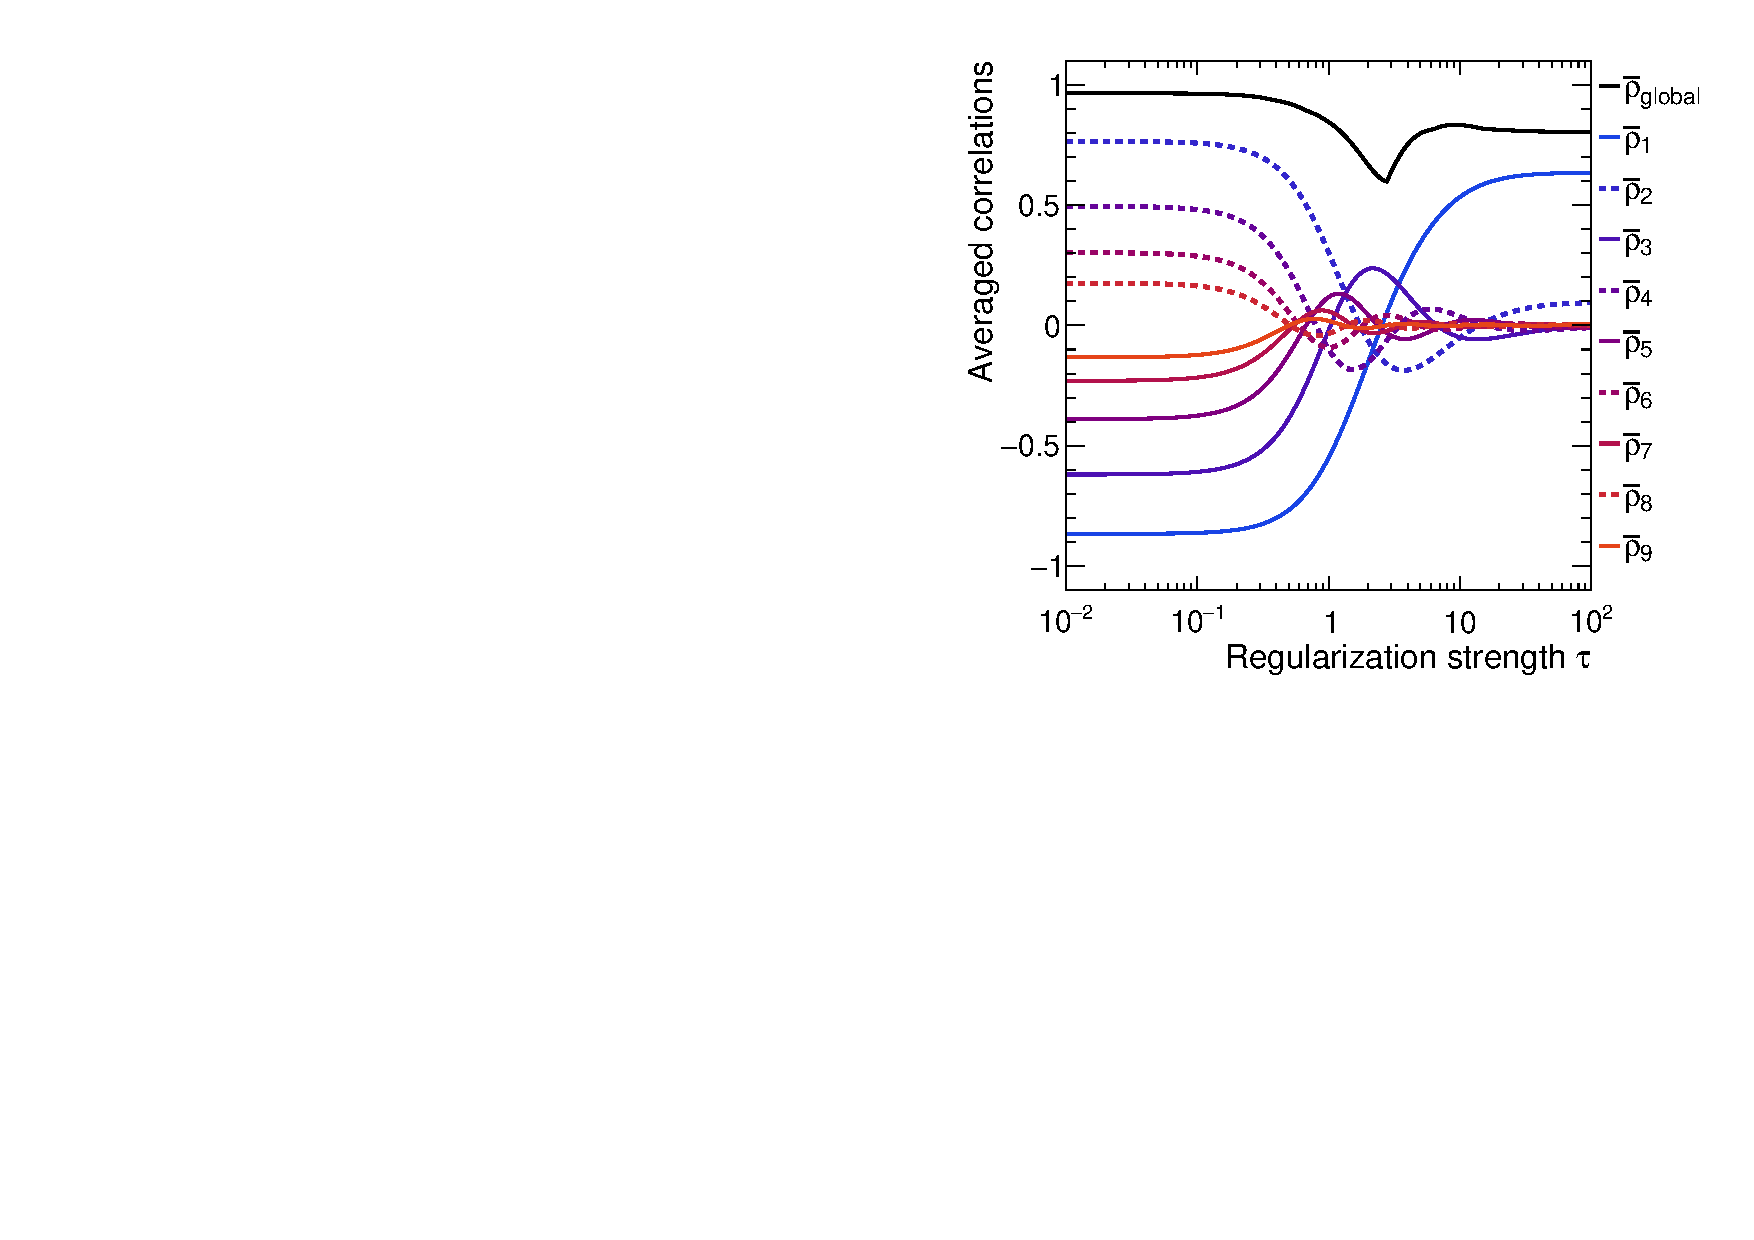
\includegraphics[width=0.48\textwidth]{figures/technique/scanTau.pdf}}\hspace{0.03\textwidth}
\subfloat[\label{fig:technique-tauscan-result}]{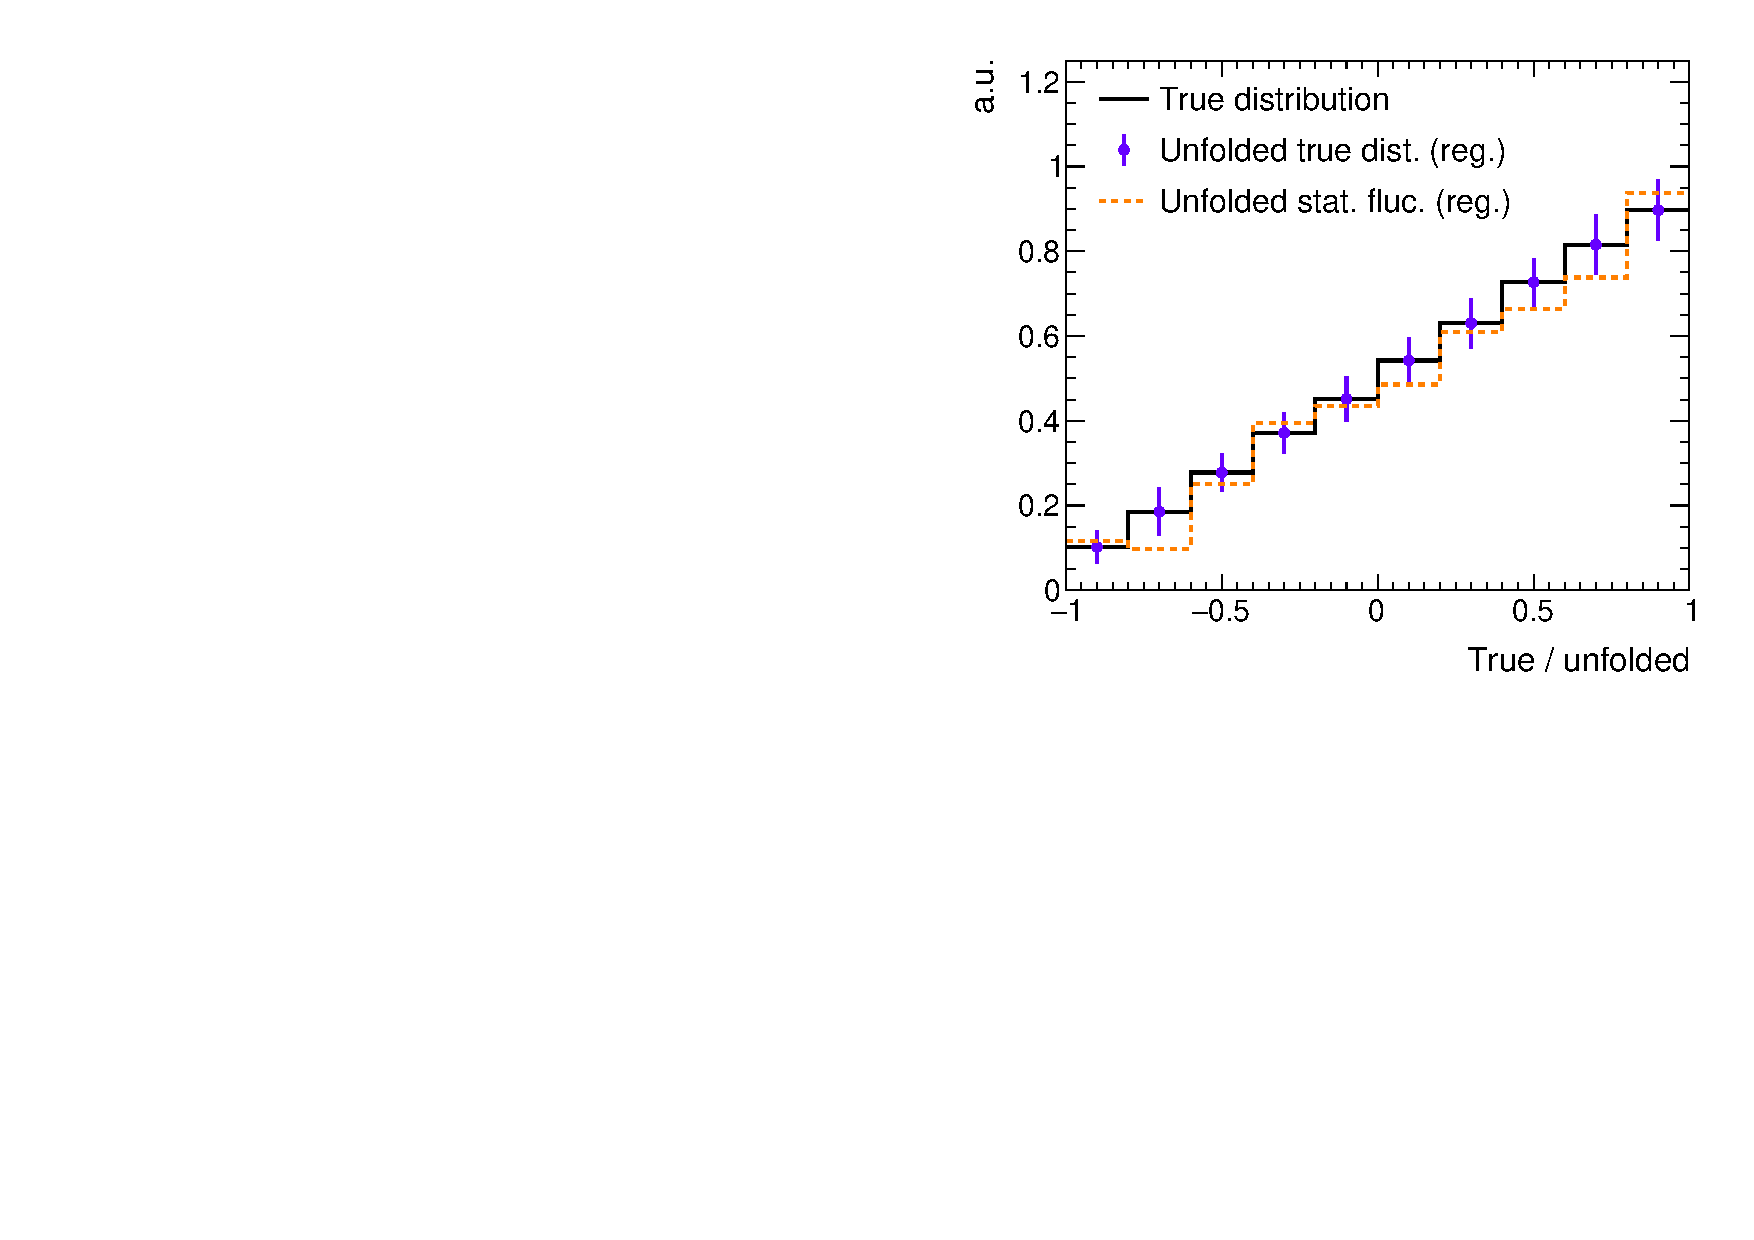
\includegraphics[width=0.48\textwidth]{figures/technique/unfoldDist.pdf}}
}

In conclusion, unfolding is an ill-posed problem which requires regularization to obtain meaningful results that are stable against statistical fluctuations. The \TUNFOLD package regularizes the response matrix by suppressing solutions with large curvatures. The procedure induces bin-by-bin correlations as a function of the amount of regularization. A trade-off between large correlations is achieved by adjusting the regularization strength to the minimum of the average global correlation coefficient.


